\chapter{Intensity modulation, direct detection}
\label{ch:imdd}

\section{What IM/DD means}

Almost every short-reach datacenter link still uses the same basic deal with
physics: put data on optical \emph{power}, and recover it with a photodiode.
That is \term{IM/DD}: \emph{intensity modulation, direct detection}. The
transmitter encodes bits as changes in optical intensity; the receiver is a
photodiode plus a transimpedance amplifier (TIA) that turns photocurrent back
into voltage. There is no local oscillator and no coherent mixing.\sidenote{Contrast
with \term{coherent} detection, which mixes the signal against a local-oscillator
laser to recover amplitude \emph{and} phase. Coherent wins for long-haul spectral
efficiency; IM/DD wins on cost and power for short reach.} Detection is
square-law (photocurrent proportional to optical power), so phase is discarded.
That limitation is acceptable inside the rack and across a few hundred meters of
fiber, where cost, power, and latency matter more than spectral efficiency. It is
why IM/DD, not coherent, wires AI compute fabrics today.

\section{The IM/DD transceiver chain}
\label{sec:txrx-chain}

Every pluggable module and every co-packaged engine is a rearrangement of the same
chain. Once you can name the blocks, you can place equalization, FEC, and
validation measurements without getting lost in form-factor jargon.

\begin{description}
\item[Transmit] laser or CW source $\to$ modulator (EML, MZM, ring)
      $\to$ driver $\to$ fiber coupling (\Cref{ch:lasers,sec:eml-eam,sec:simzm,sec:siring}).
\item[Channel] fiber, connectors, MUX (\Cref{sec:optical-channel,sec:wdm-hardware}).
\item[Receive] photodiode $\to$ TIA (optional CTLE) $\to$ SerDes/CDR or linear ADC to
      host (\Cref{sec:pd-tia,sec:equalization}).
\item[Digital] KP4 FEC in host or retimer (\Cref{sec:kp4}); module DSP optional
      (\Cref{sec:pluggables,sec:conditioning,tab:placement}).
\end{description}

The rest of this chapter fills in modulation physics, equalization, FEC, and the
modulator platforms. Noise math and measurement practice live in
\Cref{ch:models,ch:validation}.

\subsection{A pluggable link, end to end}
\label{sec:link-chain}

The block list above is one module. A working rack-to-rack link chains two of them
back to back across a fiber, and it helps to trace a single bit through the whole
path once. \Cref{fig:link-chain} follows that path as a folded loop: the transmit
side runs left to right across the top, the fiber turns the corner on the right,
and the receive side runs back along the bottom into the far switch.

Start at the switch ASIC in rack~A. It builds Ethernet frames, runs the
reconciliation and coding sublayers, and encodes KP4 FEC (\Cref{sec:phy-stack,sec:kp4}),
then hands parallel bit streams to the host \term{SerDes}. The SerDes serializes each
stream to a 112~GBd PAM4 lane, applies transmit FFE, and drives the host PCB and the
module cage connector. That electrical hop, host to module, is the AUI (an OIF VSR-class
channel; \Cref{sec:reach,sec:224g}). Inside the module, an optional DSP or retimer
reshapes the lane, or for a linear pluggable (LPO) nothing does and the host SerDes
owns the whole electrical budget (\Cref{sec:equalization,sec:224g-deploy}). The driver
then swings a modulator, an EML, Mach-Zehnder, or ring
(\Cref{sec:eml-eam,sec:simzm,sec:siring}), and electrons become photons. That is the
first domain crossing, marked E$\to$O in the figure.

The fiber plant is the quiet middle: duplex or parallel single-mode fiber, connectors,
and patch panels carrying the light a few meters to a few hundred meters
(\Cref{sec:optical-channel,sec:reach}). At the far module the light hits a photodiode
and TIA and becomes current again (O$\to$E, the second crossing;
\Cref{sec:pd-tia}). An optional module DSP cleans it up, and the rack~B host SerDes
recovers timing, equalizes the lane, and decodes KP4. The switch ASIC reassembles
frames and forwards them into the fabric, out a NIC, and over the in-node link
(PCIe or an NVLink-class fabric) into the destination GPU or CPU. Every pluggable
link is this shape; form factors and CPO only rearrange where the boundaries fall.

\begin{figure}[ht]
\centering
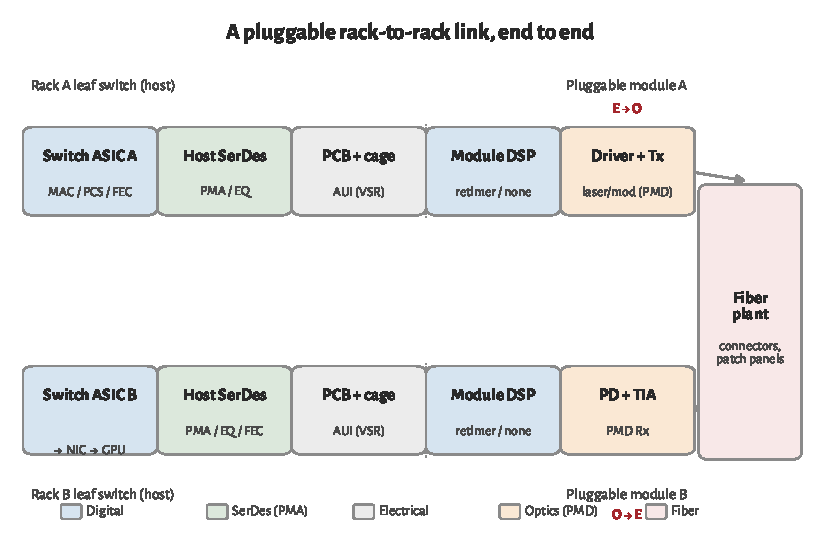
\includegraphics[width=\linewidth]{figures/fig_link_chain.pdf}
\caption{A pluggable rack-to-rack link, drawn as a folded loop. Transmit runs left to
right (switch ASIC $\to$ host SerDes $\to$ cage/AUI $\to$ module DSP $\to$ driver and
optics), the fiber turns the corner, and receive runs back into the far switch, then on
to the NIC and GPU. Colors mark the domain of each block; the two E$\leftrightarrow$O
crossings sit at the optics.\label{fig:link-chain}}
\end{figure}

This is the \emph{scale-out} path, the rack-to-rack Ethernet fabric where optics
already dominate. The \emph{scale-up} fabric that ties GPUs together
(NVLink- or UALink-class; \Cref{sec:scale-up-out}) is a different link. Its reach is
much shorter, so most of it is still copper: direct-attach cable or backplane under
roughly a meter, with no optics in the path at all. Optics only appears once rack
densification pushes those links past the copper wall, and even then it borrows the
same IM/DD building blocks over a different link and protocol layer. So the chain in
\Cref{fig:link-chain} is the one that carries the optical volume today; scale-up is
where optics is arriving next.

\section{Reach regimes, and the scope of this book}
\label{sec:reach}

``Optical interconnect'' is a wide phrase. A die-to-die link of a few millimeters
and a 10~km campus span both move bits on light, but they solve different
problems with different physics. AI compute fabrics live at the short end of that
spectrum, where lasers, IM/DD, and validation dominate cost, power, and
reliability. This book stays there and largely sets aside the 2--10~km campus and
data-center-interconnect links that have moved toward coherent optics.

\begin{table*}[ht]
\refstepcounter{table}\label{tab:reach}%
\centering
\setlength{\tabcolsep}{6pt}%
\begin{tabular}{@{}p{0.22\linewidth}p{0.18\linewidth}p{0.54\linewidth}@{}}
\toprule
Regime & Distance & Notes \\
\midrule
In-package / die-to-die & mm--cm & optical I/O chiplets (e.g. \Cref{sec:cwwdm}) \\
Chip-to-chip / co-packaged & cm & CPO engines on the switch/XPU substrate \\
Scale-up (rack scale) & $\sim$1--10~m & XPU-to-XPU; copper below $\sim$1--2~m, optics beyond \\
Intra-rack / intra-row & up to $\sim$100--500~m & SR over MMF; DR single-mode \\
\midrule
Campus / DCI \emph{(out of scope)} & 2~km (FR), 10~km (LR), and beyond & increasingly coherent, not IM/DD \\
\bottomrule
\end{tabular}
\par\medskip
{\raggedright\footnotesize\textbf{Table~\thetable.} Reach regimes. This book focuses on the top four.\par}
\end{table*}

The dividing line is roughly where a link leaves the compute fabric. Inside that
boundary, from millimeters in-package out to a few hundred meters, IM/DD is the
workhorse and the laser is the component that gates scale. That is the territory
this book treats.

\section{Where coherent takes over}
\label{sec:coherent-boundary}

\subsection{The two detection schemes, in one paragraph}

\term{IM/DD} encodes bits as changes in optical intensity and recovers them with a
square-law photodiode. Phase and polarization are discarded at detection. Coherent
detection mixes the received field against a narrow-linewidth local-oscillator (LO)
laser on a balanced photodiode pair, recovering amplitude and phase on both
polarizations. The receiver digitizes in-phase and quadrature samples and runs heavy
DSP: carrier recovery, polarization demux, chromatic dispersion compensation, and
soft-decision FEC. The coherent transmitter typically needs an I/Q modulator (or
equivalent) under the same linewidth discipline. That stack buys spectral
efficiency and reach tolerance. It costs extra photonic parts, ADC/DSP die area,
power, and latency.

\subsection{Why short reach stays IM/DD}

Inside the compute fabric, from millimeters in-package out to a few hundred meters
of single-mode fiber, loss and dispersion are modest: standard G.652.D fiber runs
about 0.2~dB/km at 1550~nm with a zero-dispersion wavelength near 1310~nm, so a
few hundred meters costs well under a decibel~\cite{itufiber}. A PAM4 IM/DD link
with equalization, FEC, and a reasonable laser closes without coherent mixing. The
energy argument from \Cref{ch:firstprinciples} applies directly: IM/DD keeps the
expensive digital work at the electrical ends where process scaling helps, and the
optical path is passive fiber. Rack and row runs also lean on bend-insensitive
G.657 fiber in patch panels and shelves, and the SR/DR reach classes below map onto
the OM4/OM5 multimode and OS1/OS2 single-mode cabling classes that ISO/IEC 11801
and TIA-492 define for the datacenter plant~\cite{fibercabling}. Retimed 800G
pluggables run roughly 14--18~W; LPO trims to roughly 7--9~W by deleting module
DSP~\cite{lpo}. A 400ZR-class coherent pluggable is built around a coherent DSP
that alone draws roughly 5--8~W inside a 15~W module budget~\cite{oif400zr},
landing near 45~pJ/bit at 400~Gb/s. Over a 100~m rack link that extra DSP power
does not buy enough margin to justify the BOM and service complexity
(\Cref{sec:power}).

\subsection{What coherent buys, and its price}

Coherent wins where the channel is harder: kilometers of fiber, amplified DWDM, and
dispersion that would crush a directly modulated PAM4 eye. Polarization multiplexing
and higher-order QAM raise bits per symbol. Electronic dispersion compensation
removes the need for tight wavelength and chirp control on the transmit laser. LO
mixing gives a sensitivity boost that IM/DD only matches with more launched power.
The price is upfront: linewidth requirements on both the transmit laser and the LO
(often well below 100~kHz for long reach), I/Q modulators or integrated coherent
PICs, high-speed ADCs, and a DSP that dominates module power. OIF standardized
400ZR coherent pluggables with a 15~W module budget for DCI spans to roughly
120~km~\cite{oif400zr}. ZR+ variants push reach further at similar or higher
power. That trade is right for campus and metro DCI. It is not the default inside
an AI rack.

\subsection{The crossover, and where it is moving}

Today the practical line sits near 2~km: intra-datacenter DR and shorter hops stay
IM/DD (\Cref{sec:reach,tab:ieee-lane}); campus FR/LR and DCI have moved to coherent
400ZR/ZR+ (\Cref{tab:reach}). Pressure pushes coherent inward on per-lane rates: at
224G and especially 448G the IM/DD SNR and TDECQ margin tighten, and some proposals
explore coherent-lite or coherent receivers for the longest scale-out
hops~\cite{cei448,e4ai448}. Pressure keeps IM/DD dominant for AI compute: LPO and
CPO attack the power wall (\Cref{sec:power,sec:224g-deploy}) by stripping module
DSP and shortening electrical reach, not by adding an LO and ADC chain. For
inference fabrics at in-package to a few hundred meters, IM/DD remains the workhorse
through the 224G generation. The open question is 448G and beyond: whether the
last scale-out meters stay PAM4/PAM6 IM/DD or whether a stripped coherent option
appears for links that already run retimed modules today (\Cref{sec:448g}).

\section{PAM4: more bits per symbol}

Through the 10G and early 25G eras, most short-reach optics used two-level NRZ:
one eye, one decision threshold, simple receivers. As per-lane rates climbed past
about 50~Gb/s, keeping NRZ would have demanded more electrical bandwidth than
connectors and SerDes could afford. The industry answer was \term{PAM4}: four
amplitude levels carrying two bits per symbol. Line rates below are in gigabaud
(\term{GBd}\firstterm{GBd}); host I/O is built in \term{SerDes}\firstterm{SerDes}
blocks.

\begin{table}[ht]
\centering
\caption{Per-lane rates and symbol rates (PAM4).\label{tab:pam4-rates}}
\begin{tabular}{@{}lll@{}}
\toprule
Per-lane rate & Symbol rate & Context \\
\midrule
100G/lane & $\approx$53.1~GBd & 400G/800G today \\
200G/lane & $\approx$106--112~GBd & 800G/1.6T ramp \\
224G/lane & $\approx$112~GBd (CEI-224G) & next SerDes generation \\
\bottomrule
\end{tabular}
\end{table}

PAM4 halves the required bandwidth versus NRZ for a given bit rate, but it costs
about 9.5~dB of SNR (three eyes instead of one, spaced one-third as far apart).
That SNR hit is why modern links assume equalization, DSP, and forward error
correction as part of the architecture rather than as optional polish
(\Cref{sec:equalization}). Looking ahead, the 448G debate is partly about whether
to stay on PAM4 at still higher baud or move to PAM6/PAM8 to ease the electrical
channel (\Cref{sec:448g}).

\section{Equalization and clock recovery}
\label{sec:equalization}

Once PAM4 became the default, the electrical channel stopped looking like a wire
and started looking like a filter. PCB traces, connectors, and cables low-pass
the signal; the receiver must undo that inter-symbol interference (ISI)\firstterm{ISI} before
slicing. Three equalizer classes appear in every short-reach link, plus clock
recovery when the bit clock is rebuilt.

\begin{description}
\item[CTLE (continuous-time linear equalizer)] \firstterm{CTLE} provides analog
      high-frequency boost, often a zero-pole pair in the SerDes front-end, the TIA,
      or a redriver chip. CTLE is cheap and low latency but fixed: it cannot adapt
      tap-by-tap to an arbitrary channel.
\item[FFE (feed-forward equalizer)] \firstterm{FFE} is a finite-impulse-response
      filter with pre- and post-cursor taps. Host SerDes and module DSPs use FFE
      (often with CTLE ahead of it) to open the eye.
      Transmitter and dispersion eye closure quaternary (TDECQ)\firstterm{TDECQ} applies a
      \emph{bounded} reference FFE when scoring transmitters (\Cref{sec:tdecq}).
\item[DFE (decision-feedback equalizer)] \firstterm{DFE} cancels post-cursor ISI
      using past symbol decisions. CEI electrical eye budgets reference an 8-tap DFE
      at the slicer (\Cref{sec:eye-budget}). DFE adds latency and error propagation
      but recovers more ISI than FFE alone at high loss.
\item[CDR (clock-data recovery)] \firstterm{CDR} extracts bit timing from the
      data stream and re-samples the eye. A \emph{retimer} includes CDR plus
      equalization and regenerates a clean output; a \emph{redriver} has CTLE/VGA but
      no CDR (\Cref{sec:conditioning}).
\end{description}

Where these blocks sit depends on the module style (\Cref{sec:pluggables,ch:networking}):

\begin{itemize}
\item \textbf{Fully retimed pluggable:} host SerDes $\to$ connector $\to$ module DSP
      (FFE/DFE/CDR) $\to$ optical engine. The module cleans a bad electrical channel.
\item \textbf{Redriver / ACC:} CTLE (+ VGA) in the cable or mid-channel; host SerDes
      still owns CDR and heavy EQ.
\item \textbf{LPO:} no module DSP/CDR. Host SerDes EQ and FEC must survive the full
      path; module may add only CTLE in the TIA and a linear driver
      (\Cref{sec:conditioning}). Optical TDECQ and electrical margin both tighten.
\end{itemize}

\Cref{fig:eq-chains} shows the correct SerDes equalizer order, then where those
blocks live in a retimed module versus LPO.

\begin{figure}[ht]
\centering
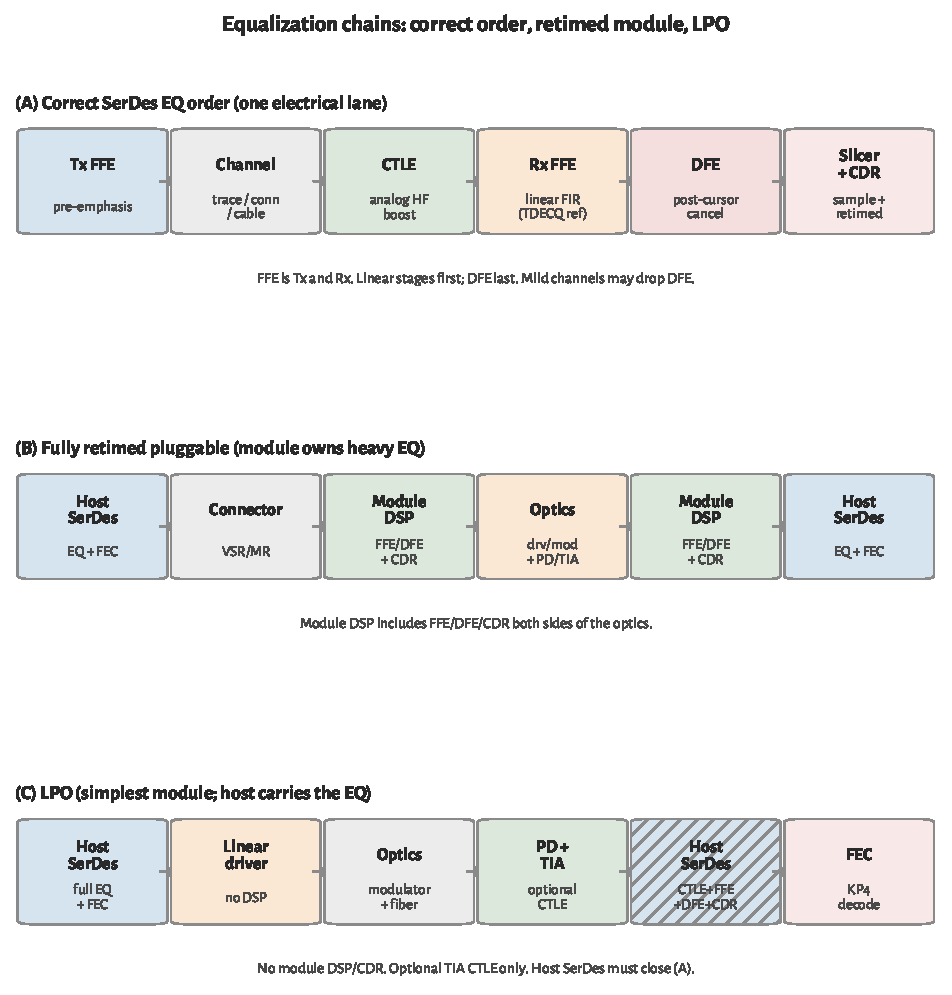
\includegraphics[width=\linewidth]{figures/fig_eq_chains.pdf}
\caption{Equalization chains. (A)~Correct order on one electrical lane: Tx FFE,
channel, CTLE, Rx FFE, DFE, then slicer/CDR. (B)~Fully retimed pluggable: module
DSP owns FFE/DFE/CDR on both sides of the optics. (C)~LPO: no module DSP; the host
SerDes must close the full EQ and FEC path.\label{fig:eq-chains}}
\end{figure}

\keyidea{CTLE boosts analog bandwidth; FFE/DFE cancel ISI digitally; CDR rebuilds
timing in retimers. LPO deletes the module-side safety net, so host equalization and
KP4 margin (\Cref{sec:kp4}) become the whole electrical story.}

\section{SerDes and DSP: who does the work}
\label{sec:serdes-dsp}

The equalizers above have to run somewhere, and ``SerDes'' and ``DSP'' get used
loosely for that somewhere. They are not the same thing, and at 112~GBd the line
between them has mostly dissolved. Pinning down the vocabulary makes the retimed
versus LPO versus CPO argument (\Cref{sec:conditioning,ch:networking}) concrete
instead of a wall of acronyms.

\subsection{What the SerDes is}

\term{SerDes} is the high-speed electrical I/O macro on an ASIC: switch silicon, a
NIC, an accelerator, or a module chip. On transmit it serializes wide, slow
parallel data from the MAC/PCS into one PAM4 lane on the wire; on receive it
deserializes the sampled lane back to parallel words. That is the literal
serializer/deserializer job. Everything else the SerDes does is in service of
getting a clean symbol stream across a lossy channel.

\subsection{Analog SerDes versus DSP-based SerDes}

How the SerDes conditions the signal splits into two design styles. An
\emph{analog} (mixed-signal) SerDes equalizes in the analog domain (CTLE, a few
analog FFE/DFE taps) and slices directly. It is low power and low latency but
limited in how much loss it can undo and how flexibly it adapts. A
\term{DSP-based}\firstterm{dspserdes} SerDes puts a high-speed ADC on the receive
lane, digitizes the eye, and does FFE, DFE, and timing recovery numerically, with
a DAC and digital pre-distortion on transmit. It burns more power and adds
latency, but it closes far more channel loss and adapts tap-by-tap. Above roughly
50~GBd the DSP-based architecture won: 112~GBd (224G) host SerDes and module
retimers are ADC/DSP designs. So the ``DSP'' that cancels ISI at 224G usually lives
\emph{inside} the SerDes, not in a separate chip.

\subsection{Two things people call ``the DSP''}

That is the first meaning of DSP: the digital equalization and clock recovery
inside a modern SerDes. The second meaning is \emph{the module DSP}, a distinct
retimer chip in a pluggable that has its own ADC/DSP SerDes on the host side, an
FFE/DFE/CDR core, a gearbox (\Cref{sec:gearbox}), and often the FEC engine, then
drives the optics. When the book says a retimed module ``has a DSP'' and LPO
``deletes the DSP'' (\Cref{sec:conditioning}), it means this second chip. Deleting
it does not delete DSP from the link; it moves the equalization burden back onto
the \emph{host} SerDes DSP and onto FEC.

\subsection{Where FEC sits}

FEC is a third block, and it is usually not part of the SerDes proper. KP4 encode
and decode live in the PCS/FEC layer on the host (or in the module DSP when one is
present), operating on the recovered symbol stream (\Cref{sec:kp4}). This is why a
link can have a healthy SerDes eye and still fail on FEC, or ride an ugly eye that
KP4 cleans: the SerDes recovers symbols, FEC fixes what is left. Validation reads
pre-FEC BER exactly at that SerDes-to-FEC boundary.

\subsection{Mapping it back to module styles}

\Cref{tab:serdes-dsp} sorts the blocks by where they physically run for the three
module styles. \Cref{fig:eq-chains} shows the same split as signal chains. Read the
LPO column as the design point that matters most for AI power budgets: the host
SerDes DSP and host FEC carry the entire electrical channel, because the module has
no retimer to hide behind (\Cref{sec:224g-deploy}).

\begin{table}[ht]
\centering
\caption{Where each block runs, by module style.\label{tab:serdes-dsp}}
\setlength{\tabcolsep}{4pt}%
\footnotesize
\begin{tabular}{@{}p{0.24\linewidth}p{0.22\linewidth}p{0.20\linewidth}p{0.22\linewidth}@{}}
\toprule
Block & Retimed & LPO & CPO (XSR) \\
\midrule
Serialize / PAM4 & Host SerDes & Host SerDes & Host SerDes \\
Rx EQ (FFE/DFE) & Module DSP & Host SerDes DSP & Host SerDes DSP \\
CDR / retiming & Module DSP & Host SerDes & Host SerDes \\
KP4 FEC & Host (or module) & Host & Host \\
Optical drive & Module DSP out & Linear driver & On-package engine \\
\bottomrule
\end{tabular}
\end{table}

\keyidea{The SerDes is the ASIC's electrical PHY; at 224G its equalization and clock
recovery are done in DSP inside the SerDes. ``The module DSP'' is a separate
retimer chip. LPO removes that retimer, so the host SerDes DSP plus KP4 FEC
(\Cref{sec:kp4}) own the whole electrical channel. Optics begin only after that
handoff.}

\section{The Ethernet PHY stack: where optics attaches}
\label{sec:phy-stack}

The SerDes, the FEC, and the optics are not loose parts. IEEE 802.3 stacks them into
named sublayers, and knowing the stack tells you exactly where the optical
transceiver plugs in and which block owns each impairment. Ethernet lives at the
bottom two OSI layers: the \term{MAC}\firstterm{MAC} (data link) builds frames and carries the
addressing, and the \term{PHY}\firstterm{PHY} (physical) turns those frames into
signals on the wire. Everything in this book sits inside the PHY.

\subsection{The sublayers, top to bottom}

The PHY is itself a stack. \Cref{tab:phy-stack} lists the sublayers a 400G/800G port
walks through on transmit (receive runs in reverse).

\begin{table}[ht]
\centering
\caption{IEEE 802.3 PHY sublayers, transmit order.\label{tab:phy-stack}}
\setlength{\tabcolsep}{4pt}%
\footnotesize
\begin{tabular}{@{}p{0.14\linewidth}p{0.52\linewidth}p{0.24\linewidth}@{}}
\toprule
Sublayer & Function & Domain \\
\midrule
MAC & Frame, address, CRC & Digital, host \\
RS & Reconciliation: adapt MAC to the PHY across the xMII & Digital, host \\
PCS & 64B/66B, 256B/257B transcode, scramble, RS-FEC & Digital \\
PMA & Serialize, lane mux, clock recovery (SerDes) & Mixed-signal \\
PMD & Modulate/detect light: laser, driver, PD, TIA & Optical \\
\bottomrule
\end{tabular}
\end{table}

Two interface names sit between these blocks and cause most of the confusion. The
\term{xMII}\firstterm{xMII} (for example 400GMII) is a wide parallel bus inside the
chip between MAC and PCS. The \term{AUI}\firstterm{AUI} (for example 400GAUI-4) is the
electrical serial lane set that leaves the host and crosses the faceplate connector
to the module. The AUI is the CEI electrical channel your SerDes has to survive
(\Cref{sec:serdes-dsp,ch:networking}); the \term{PMD}\firstterm{PMD} is the optical
transceiver on the far side of it.

\subsection{Where the optics attaches}

Optics is the PMD, and only the PMD. Everything above it is electrical or logical and
is medium-independent: the same MAC, RS, PCS, and PMA feed a copper DAC, a
multimode SR module, or a single-mode DR module. That is the whole point of the
layering. When IEEE names \texttt{400GBASE-DR4} or \texttt{800GBASE-DR8}, it is
naming a PMD (\Cref{sec:pmd-reach}); the digital stack above is shared. It is also
why the retimed-versus-LPO-versus-CPO argument is really about \emph{where the PMA
and PCS/FEC physically sit} relative to the AUI, not about changing the optics
(\Cref{sec:serdes-dsp}).

\subsection{Line-rate accounting}

The layering is where the MAC-rate-versus-line-rate gap (\Cref{tab:rate-stack})
actually comes from. Take one 400G port. The MAC delivers 400~Gb/s of payload. The
PCS transcodes it (256B/257B adds about 0.4\%) and then RS(544,514) FEC adds 30
parity symbols per 514 data symbols, a $544/514$ expansion of roughly 5.8\% relative
to payload (equivalently 5.5\% of the coded line, \Cref{sec:kp4}). The two multiply
out to $257/256 \times 544/514 = 1.0625$, so the line carries $400 \times 1.0625 =
425$~Gb/s, split as four AUI lanes at 106.25~Gb/s (53.125~GBd PAM4). The optical PMD
carries that same 425~Gb/s. So ``400G Ethernet'' is a 400~Gb/s MAC rate riding a
425~Gb/s line, and the extra 25~Gb/s is transcode plus FEC, not wasted bandwidth.

\subsection{What the PCS actually does}

Inside the PCS\firstterm{PCS}, the MAC's 64-bit words are first wrapped in 64B/66B blocks: a 2-bit
sync header (\texttt{01} for data, \texttt{10} for control) lets the receiver find
block boundaries in the serial stream. Four 66-bit blocks are then transcoded into
one 257-bit block, which compresses the four 2-bit sync headers to a single bit and,
crucially, produces a 256-bit payload that aligns cleanly with 10-bit RS-FEC symbols
($\mathrm{lcm}(256,10)=1280$, so five blocks make exactly 128 symbols with no
remainder). The RS(544,514) encoder then adds parity (\Cref{sec:kp4}), and the PMA
distributes the coded symbols across logical lanes, bit-multiplexes them down to the
physical AUI lanes, and serializes each to PAM4. The payload bits themselves are
never altered by transcoding; only the framing overhead is squeezed.

Where these blocks physically live is an implementation choice, not a layer rule.
The PCS/FEC can sit in the host switch ASIC or in a module retimer DSP; LPO deletes
the module DSP and forces the host to own PCS/FEC and all of the PMA equalization
(\Cref{sec:serdes-dsp,sec:conditioning}). The layer names stay the same regardless of
which chip runs them.

\keyidea{Ethernet is MAC (frames) plus PHY, and the PHY is RS, PCS, PMA, PMD.
Optics is only the PMD; everything above is medium-independent, which is why one
digital stack feeds copper, multimode, or single-mode. The MAC-to-line-rate gap is
transcode ($257/256$) times FEC ($544/514$), giving 425~Gb/s on a 400G port. The
module-style debate is about which side of the AUI runs the PMA and PCS/FEC.}

\section{Test points: where the link is measured}
\label{sec:test-points}

Every metric in this book is taken \emph{somewhere}. A datasheet line like
``TDECQ~$\le$~3.4~dB'' or ``stressed sensitivity $-3.1$~dBm'' means nothing until you
name the reference plane it was measured at. The standards name those planes TP0
through TP5, plus the host-referenced pair TP1a and TP4a, and they run in order from
the transmit silicon to the receive silicon. Learning them turns a scattered pile of
numbers into a map: each spec belongs to exactly one plane, and each plane is owned
by one document. \Cref{fig:test-points} walks the chain; \Cref{tab:test-points}
is the lookup card.

The mistake to avoid is treating TP2 and TP3 as electrical points just past a
connector. They are \emph{optical} planes at the fiber. TP2 is the light launched
into the fiber, measured after the module's electrical-to-optical conversion (driver
plus laser or modulator). TP3 is the light arriving at the far module, before its
optical-to-electrical conversion (photodiode plus TIA). The electrical planes are the
ones on either side of those two crossings.

\begin{figure}[ht]
\centering
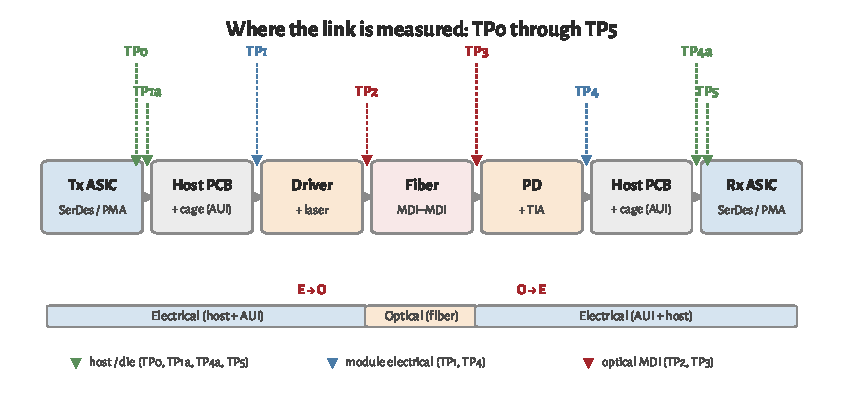
\includegraphics[width=\linewidth]{figures/fig_test_points.pdf}
\caption{Test points on a one-way IM/DD link. Green marks the host and die-pad
electrical planes (TP0, TP1a, TP4a, TP5); blue the module's electrical connector
(TP1, TP4); red the optical planes at the fiber \term{MDI} (TP2, TP3).
The two domain crossings, E$\to$O in the module transmitter and O$\to$E in the module
receiver, sit between the electrical and optical planes.\label{fig:test-points}}
\end{figure}

\newthought{Read the chain in order.} At the transmit end, \textbf{TP0} is the
transmit SerDes output at the die pad, the silicon designer's reference. \textbf{TP1a}
is the same host signal referenced at the module cage, the \term{AUI} the module must
accept; its electrical eye quality is \term{EECQ}\firstterm{EECQ}, the electrical
analog of TDECQ. \textbf{TP1} is the module's electrical input on the far side of the
mated connector. The module then converts electrical to optical, and \textbf{TP2} is
the optical launch at the transmitter \term{MDI}\firstterm{MDI}, where TDECQ, TECQ, OMA$_{\mathrm{outer}}$,
ER, and RIN are specified (\Cref{ch:validation,sec:tdecq}). After the fiber,
\textbf{TP3} is the optical input at the receiver MDI, where stressed receiver
sensitivity (SECQ) is specified. The module converts back to electrical at
\textbf{TP4} (its electrical output), \textbf{TP4a} is the host-referenced input near
the receive SerDes under worst-case module output, and \textbf{TP5} is the receive
die pad.

\begin{table*}[ht]
\refstepcounter{table}\label{tab:test-points}%
\centering
\setlength{\tabcolsep}{5pt}%
\footnotesize
\begin{tabular}{@{}p{0.05\linewidth}p{0.075\linewidth}p{0.29\linewidth}p{0.30\linewidth}p{0.15\linewidth}@{}}
\toprule
Point & Domain & Location & Principal measurement & Owning spec \\
\midrule
TP0 & Electrical & Tx ASIC/SerDes die pad (host) & Silicon Tx quality; design reference, hard to probe once packaged & OIF CEI C2M \\
TP1a & Electrical & Host output at the cage, host-referenced (SerDes output via a host compliance board) & Host Tx eye, EECQ; the AUI the module must accept & OIF CEI C2M; LPO MSA \\
TP1 & Electrical & Module electrical input (module side of the mated connector) & Module input stressor calibration & IEEE 802.3 AUI; OIF CEI \\
TP2 & Optical & Transmitter MDI, fiber launch (after E$\to$O) & TDECQ, TECQ, OMA$_{\mathrm{outer}}$, ER, RIN$_x$OMA & IEEE 802.3 PMD; LPO MSA \\
TP3 & Optical & Receiver MDI, fiber input (before O$\to$E) & Stressed receiver sensitivity, SECQ & IEEE 802.3 PMD; LPO MSA \\
TP4 & Electrical & Module electrical output (module side of the connector) & Module Rx electrical output, EECQ & IEEE 802.3 AUI; OIF CEI \\
TP4a & Electrical & Stressed host input, host-referenced (near the Rx SerDes) & Host Rx under worst-case module output & OIF CEI C2M; LPO MSA \\
TP5 & Electrical & Rx ASIC/SerDes die pad (host) & Silicon Rx recovery; design reference, hard to probe & OIF CEI C2M \\
\bottomrule
\end{tabular}
\par\medskip
{\raggedright\footnotesize\textbf{Table~\thetable.} Test-point reference planes on a
short-reach IM/DD link, transmit to receive. The optical planes TP2 and TP3 carry the
transmitter- and receiver-quality specs; the electrical planes carry the host and
module eye specs. See \Cref{tab:lpo-tp} for the concrete LPO MSA assignments.\par}
\end{table*}

\newthought{Who owns which plane.} The split is not arbitrary. IEEE 802.3 optical PMD
clauses define the transceiver planes: the optical TP2 and TP3, and the module's
electrical PMD input and output at TP1 and TP4~\cite{ieee8023dj}. The OIF Common
Electrical I/O chip-to-module work owns the electrical planes deeper into the host:
the die pads TP0 and TP5, and the host-referenced compliance points TP1a and TP4a,
which are measured through host and module compliance boards to de-embed the
fixture~\cite{cei224}. The LPO MSA then binds both sides into a single product
contract for a DSP-less module, with the six-point ladder (TP1a, TP1, TP2, TP3, TP4,
TP4a) tabulated in \Cref{tab:lpo-tp}~\cite{lpomsa}.

The numbering is a family of conventions, not one universal set. IEEE optical PMD
clauses commonly define only TP1 through TP4, with the optical measurements at TP2
and TP3; the die pads TP0/TP5 and the host-referenced TP1a/TP4a come from the
chip-to-module electrical world. Fibre Channel historically used its own reference
points. Match the labels to the document you are reading rather than assuming a shared
TP0-to-TP5 spine.

\newthought{Where compliance testing concentrates.} Optical transmitter compliance
lives at TP2 (TDECQ, OMA, ER); optical receiver compliance lives at TP3 (stressed
sensitivity). Electrical host and module compliance concentrate at TP1a and TP4a,
which is why a module that passes optical TDECQ at TP2 can still fail interop if it
misses EECQ at TP1a. TP0 and TP5 sit inside the package and are informative for
silicon design but hard to probe in a finished system. A retimed module recovers the
signal before TP4; a linear (LPO) module does not, so at 224G its host EQ and FEC
carry the whole electrical channel (\Cref{sec:conditioning,sec:pmd-reach}).

\keyidea{The plane makes the number. TP2 and TP3 are optical, at the fiber MDI, and
carry transmitter and receiver quality (TDECQ, stressed sensitivity). TP1 and TP4 are
the module's electrical connector; TP1a and TP4a are host-referenced near the SerDes;
TP0 and TP5 are the die pads. IEEE 802.3 owns the optical planes, OIF CEI owns the
die and host-referenced electrical planes, and the LPO MSA binds all of them into one
DSP-less product contract (\Cref{tab:lpo-tp}).}

\section{The link-budget vocabulary}

These terms are the language of both datasheets and debug. Learn them as a
ledger, not as a glossary quiz: when a link fails, you are almost always arguing
about one of them.

\begin{description}
\item[OMA (optical modulation amplitude)] \firstterm{OMA} $P_1 - P_0$: the real signal swing.
      For PAM4 the ``outer OMA'' spans the outermost levels.
\item[Extinction ratio (ER)] \firstterm{ER} $P_1/P_0$, in dB. Trades against insertion loss and
      against \term{TDECQ} (\Cref{ch:validation}).
\item[RIN (relative intensity noise)] \firstterm{RIN} the laser's own amplitude noise; sets a
      noise floor that matters more as OMA shrinks.
\item[Chirp] the unwanted frequency modulation that accompanies intensity
      modulation. Large in directly modulated lasers; small and controllable in
      externally modulated lasers. See \Cref{sec:chirp-dispersion}.
\item[Chromatic dispersion penalty] dispersion $\times$ chirp $\times$ distance
      produces inter-symbol interference. This drives the wavelength plan and the
      choice between directly and externally modulated lasers (\Cref{sec:chirp-dispersion}).
\item[Receiver sensitivity] the minimum OMA needed to hit a target bit-error
      ratio; ``stressed'' sensitivity adds a calibrated impairment for margin.
\end{description}

\aside{A clean mental model: start with transmitter OMA, subtract connector and
fiber loss, subtract penalties (dispersion, TDECQ, reflection), and compare the
result to receiver sensitivity (\Cref{sec:sensitivity,ch:models,sec:link-budget}). What remains is margin.}

\section{Chirp, dispersion, and the IM/DD penalty}
\label{sec:chirp-dispersion}

IM/DD detects power, not phase, but phase still matters on the fiber. Intensity
modulation couples to frequency through the laser or modulator \emph{chirp}
parameter $\alpha$: a change in output power shifts the instantaneous optical
frequency. Single-mode fiber then converts that frequency wander into intensity
distortion via chromatic dispersion (different $\lambda$ travel at slightly
different speeds).

The penalty grows with chirp $\times$ dispersion $\times$ distance. At O-band
($\sim$1310~nm) dispersion is near zero ($|D|\lesssim 3$~ps/(nm$\cdot$km)), which is why
silicon photonics and many datacenter SMF\firstterm{SMF} links use 1310~nm class wavelengths. At
C-band ($\sim$1550~nm) dispersion is larger; chirpy sources pay more per kilometer.

Source choice sets chirp (\Cref{ch:lasers,tab:tx-modulator,sec:eml-eam}):

\begin{itemize}
\item \textbf{DML:} large $\alpha$; fine for tens of meters of MMF or uncooled SR,
      poor for FR-class SMF unless rate and reach stay short.
\item \textbf{EML / external MZM / ring:} low chirp; default for DR/FR and CPO.
\item \textbf{Reflections:} light reflected back into the laser raises effective
      chirp and RIN; optical return loss (ORL)\firstterm{ORL} specs exist for this reason
      (\Cref{sec:optical-channel}).
\end{itemize}

For the distances this book treats (in-package through a few hundred meters), dispersion
is often secondary to TDECQ, connector loss, and receiver noise. It becomes decisive
when a low-chirp assumption fails (aging EAM bias, DML on SMF, or FR edge cases).
TDECQ embeds dispersion in its name because the reference receiver includes a
dispersion penalty model for the standardized test channel.

\section{Forward error correction}
\label{sec:kp4}

Modern PAM4 links do not meet raw bit-error-ratio targets on their own; they lean
on \term{FEC}\firstterm{FEC}. The datacenter workhorse is \term{KP4}\firstterm{KP4}, a Reed--Solomon code
RS(544,514)\firstterm{RS544514} operating on 10-bit symbols. The name comes from
\texttt{100GBASE-KP4} in IEEE 802.3bj: K for backplane, P for PAM4, 4 for four
lanes~\cite{ieee8023bj}. Today ``KP4'' means that FEC code on any
PAM4 Ethernet link (optical DR, 224G SerDes, and backplane), not only the original
backplane PHY. The link is specified to a
\emph{pre-FEC}\firstterm{preFEC} BER threshold, on the order of $2.4\times10^{-4}$, which FEC then
drives down to an effectively error-free \emph{post-FEC}\firstterm{postFEC} BER.

Two consequences matter in practice:

\begin{enumerate}
\item Validation targets are stated in pre-FEC BER, and FEC symbol-error
      histograms are a rich debug signal (they reveal \emph{how} a link is
      failing, not just that it is).
\item Emerging \term{linear-drive} optics (\term{LPO}\firstterm{LPO}/\term{LRO}\firstterm{LRO}, \Cref{ch:networking}) remove
      the DSP/retimer to save power, which tightens the link budget and leans
      even harder on FEC and on transmitter quality (\Cref{sec:equalization}).
\end{enumerate}

\paragraph{KP4 in practice.}

\term{KP4} maps to Reed--Solomon RS(544,514) on 10-bit symbols: 514 payload symbols,
30 parity, up to 15 correctable symbol errors per codeword. Coding overhead is
$30/544\approx5.5\%$, so the \emph{line rate} on the wire exceeds the MAC/info rate
(for example, 802.3dj delivers $\approx$211~Gb/s payload on a 224~Gb/s PAM4 lane).
\Cref{tab:rate-stack} is the decoder for the three rate names you will see in
802.3dj and CEI-224G docs (example: one 200G Ethernet lane).

\begin{table}[ht]
\centering
\caption{Three rate names on one 802.3dj lane (200G Ethernet).\label{tab:rate-stack}}
\begin{tabular}{@{}p{0.18\linewidth}p{0.42\linewidth}p{0.32\linewidth}@{}}
\toprule
Term & Meaning & Example \\
\midrule
MAC rate & User Ethernet throughput at MAC & 200~Gb/s per lane \\
Line rate & Bits on wire incl.\ FEC overhead & $\sim$211--224~Gb/s (context-dependent) \\
Symbol rate & Baud on the electrical/optical lane & $\sim$112~GBd PAM4 \\
\bottomrule
\end{tabular}
\end{table}

The optical PHY is qualified to a \emph{pre-FEC} BER threshold, typically
$2.4\times10^{-4}$ for KP4-class links. That corresponds to $Q\approx3.5$ on the
Gaussian model of \Cref{sec:qber}. Post-FEC the target is effectively error-free
($10^{-12}$ to $10^{-15}$ class). Validation always reports pre-FEC BER during
bring-up; post-FEC confirms the decoder is working.

FEC symbol-error \emph{histograms} are a debug tool: clustered errors point to
burst impairments (reflections, power droop); sparse errors point to Gaussian noise
margin. At 448G/lane, CEI notes that KP4 at $10^{-4}$ pre-FEC may not close on
40~dB-class channels without stronger codes (\Cref{tab:448-fec}): MLC plus higher
overhead RS, or hard-decision FEC in demos (\Cref{sec:448g}).

\section{Ethernet optical PMDs and reach classes}
\label{sec:pmd-reach}

IEEE 802.3 names the optical transceiver (\term{PMD}) separately from
the MAC rate. Short-reach IM/DD classes that matter for AI fabrics:

\begin{description}
\item[SR (short reach)] \firstterm{SR} multimode fiber, VCSEL at 850~nm or evolving MMF\firstterm{MMF} solutions;
      rack and row distances; modal noise and bandwidth limit legacy SR.
\item[DR (datacenter reach)] \firstterm{DR} single-mode, typically 500~m class at 1310~nm; PAM4,
      KP4, TDECQ limits; the mainstream 400G/800G/1.6T module reach.
\item[FR (far reach)] \firstterm{FR} single-mode, 2~km class; same optics family as DR with tighter
      transmitter specs; chirp and dispersion matter more at the margin.
\end{description}

Naming examples: 400G-DR4 (four lanes), 800G-DR8, 800G-FR8 (eight $\lambda$, 2~km).
802.3dj adds 200G/lane Ethernet; the 400G/lane study group targets the next
generation (\Cref{tab:ieee-lane,sec:448g}). Campus LR and coherent DCI sit beyond
this book's scope (\Cref{tab:reach}).

\section{The per-lane roadmap: 224G and beyond}
\label{sec:224g}

Per-lane rate is the axis the whole industry advances along, because doubling it
roughly doubles switch and module capacity for the same lane count. The electrical
I/O roadmap is set by the OIF's Common Electrical I/O (CEI) projects, and optics
tracks it closely.

\begin{table}[ht]
\centering
\caption{The CEI per-lane roadmap.\label{tab:cei-roadmap}}
\begin{tabular}{@{}llll@{}}
\toprule
Generation & Per lane & Modulation & Ethernet rates \\
\midrule
CEI-112G & 112~Gb/s & PAM4 & 100/200/400G \\
CEI-224G & 224~Gb/s & PAM4 ($\approx$112~GBd) & 200/400/800/1600G \\
CEI-448G & 448~Gb/s & TBD (PAM4/6/8) & 400/800/1600/3200G \\
\bottomrule
\end{tabular}
\end{table}

\Cref{fig:cei-rate-year} puts that ladder on a longer clock: OIF CEI has roughly
doubled the rate per differential pair every four to five years since the early
2000s. Open markers for 224G and 448G follow the demo deck's ``202X'' placement;
224G is shipping now, 448G is still pathfinding~\firstcite{cei224}.

\begin{figure}[ht]
\centering
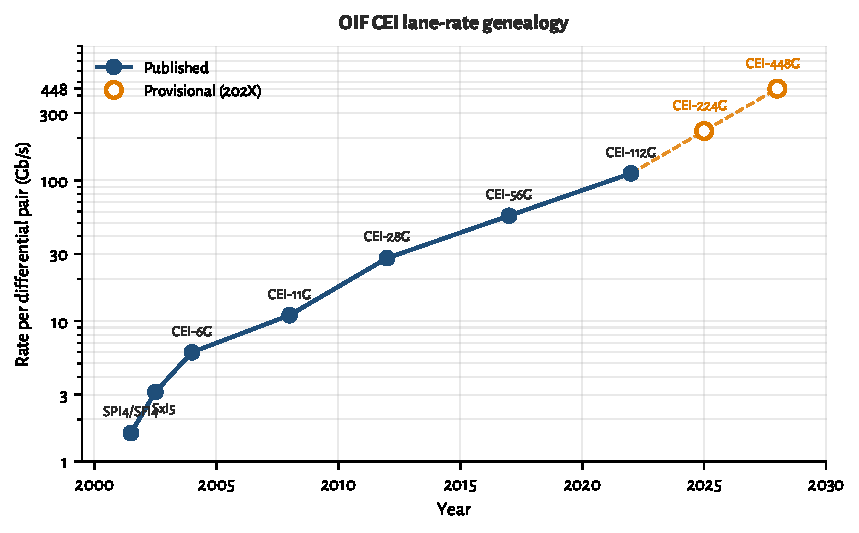
\includegraphics[width=0.92\linewidth]{figures/fig_cei_rate_vs_year.pdf}
\caption{OIF CEI rate per differential pair versus year (log scale). Data from the
OFC~2025 CEI interoperability demo genealogy; 224G/448G years are provisional
placements for the deck's 202X entries, and 448G's rate is the naming target
(PAM order still open).\label{fig:cei-rate-year}}
\end{figure}

\subsection{224G is settled; the frontier is deployment}

\term{CEI-224G} kicked off in 2022 as the electrical follow-on to CEI-112G. It
kept PAM4 and roughly doubled the baud, to about 112~GBd per lane, with reach
projects from XSR through LR now maturing. That choice is no longer the open
debate; it is the shipping baseline. Eight 224G lanes make a 1.6~Tb/s port, and
the same SerDes generation feeds 102.4~Tb/s-class switch silicon
(\Cref{sec:cpo-status}). Copper reach has collapsed to about a meter, DSP-based
SerDes are assumed, and a \term{CEI-224G-Linear} variant defines linear operation
without a DSP/retimer in the optical module: the electrical foundation for LPO
(\Cref{ch:networking}). The remaining work is deployment: closing LPO margins,
qualifying ELSFP banks for CPO, and holding yield at volume, not inventing a new
modulation alphabet.

\Cref{fig:cei-reach-map} is the reach map those projects sit on: \term{XSR}/XSR+
inside the package (die-to-die and die-to-optical-engine), \term{VSR} from ASIC to
a faceplate pluggable, \term{MR} chip-to-chip on the board (PCB or twinax), and
\term{LR} for backplane and longer copper cables~\firstcite{cei224}. The media
labels (host PCB traces, twinax, optical fiber, optical module) are where the
loss budget actually lives; the CEI class name is the electrical recipe for that
hop. \Cref{tab:cei224-reach} is the matching lookup card from the CEI-224G project
map (OFC~2025 demo framing)~\firstcite{cei224demo,cei224}.

\begin{figure}[ht]
\centering
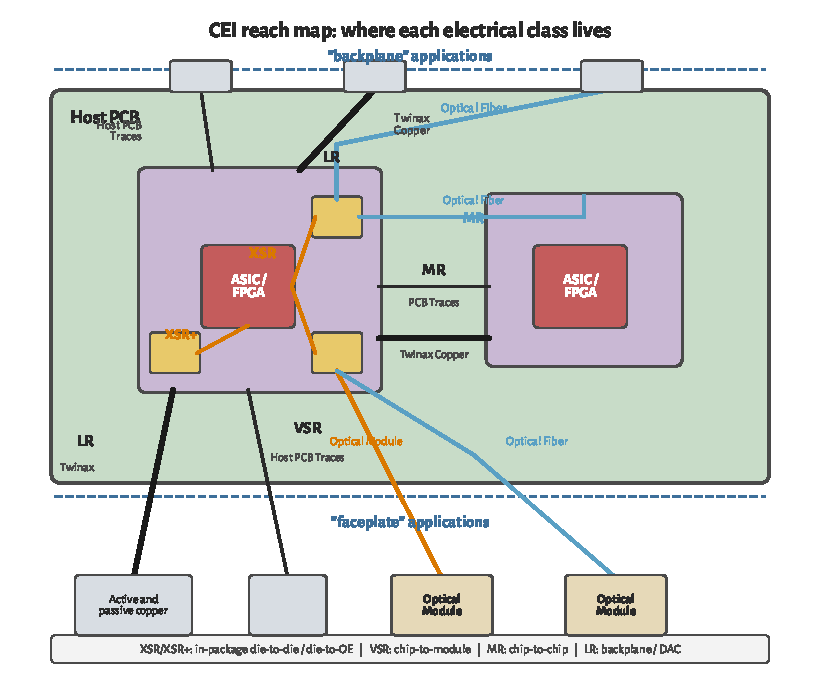
\includegraphics[width=\linewidth]{figures/fig_cei_reach_map.pdf}
\caption{CEI reach map on a host PCB (redrawn). Backplane applications sit above
the board; faceplate cages and modules sit below. XSR/XSR+ are in-package;
VSR is chip-to-module; MR is chip-to-chip; LR covers backplane and active/passive
copper.\label{fig:cei-reach-map}}
\end{figure}

\begin{table*}[ht]
\refstepcounter{table}\label{tab:cei224-reach}%
\centering
\setlength{\tabcolsep}{4pt}%
\footnotesize
\begin{tabular}{@{}p{0.12\linewidth}p{0.22\linewidth}p{0.28\linewidth}p{0.30\linewidth}@{}}
\toprule
Class & Hop & Nominal reach / channel & Notes \\
\midrule
XSR & Die-to-die or die-to-OE & $\lesssim$50~mm package substrate & CPO / chiplet optics; light EQ \\
VSR & Chip-to-pluggable module & $\sim$200~mm host + $\sim$20~mm module, 1 connector & Classic faceplate retimed path \\
MR & Chip-to-chip / midplane & $\sim$500~mm, 1 connector & Board-scale copper \\
LR & Backplane or copper cable & $\sim$1000~mm host+daughter, 2 connectors & DAC/ACC/AEC territory \\
Linear & Chip-to-linear module & Same cages as VSR-class ports; no module DSP & LPO foundation; host EQ + FEC \\
\bottomrule
\end{tabular}
\par\medskip
{\raggedright\footnotesize\textbf{Table~\thetable.} CEI-224G electrical classes (project map).
BER target on the reach classes is $10^{-15}$ or better with FEC allowed. Draft
LR/MR IAs were member-review as of OFC~2025; Linear is the separate full-linear
module track.\par}
\end{table*}

One SerDes core may not cover XSR through LR efficiently: short reaches want
simple, low-power equalization, while LR burns DSP to close tens of dB of loss.
That is why Linear is its own project rather than ``VSR with the DSP deleted,''
and why CPO (XSR) and LPO (Linear) show up as different power/serviceability bets
(\Cref{sec:224g-deploy,sec:pluggables,sec:cpo-status}).

\subsection{Deploying 224G: LPO, COM, and TDECQ corners}
\label{sec:224g-deploy}

At 224G the alphabet is settled (PAM4 + KP4). What fails in the field is the
\emph{margin stack}: electrical channel operating margin (COM) on the host side,
transmitter and dispersion eye closure quaternary (TDECQ) on the optical side,
and the production corners that couple them (\Cref{sec:prod-corners}). Retimed
modules still dominate 1.6T faceplate ports because their DSP absorbs host-channel
sin. LPO and LRO exist to delete that DSP for power and latency; they only ship
when both ledgers close without it~\firstcite{lpo,cei224,semtech224}.

\paragraph{The two ledgers that must close together.}
A retimed module can hide a bad host PCB behind module EQ. An LPO module cannot.
You therefore run two go/no-go tests as one program:

\begin{description}
\item[Electrical COM] After the CEI reference TX, channel, and Rx (CTLE + 8-tap
      DFE), COM\firstterm{COM} $\ge3$~dB is the usual pass line at the slicer
      (\Cref{sec:com,sec:eye-budget}). At 112~GBd the residual eye after that
      equalizer is only a few millivolts tall; KP4 then cleans pre-FEC BER near
      $2.4\times10^{-4}$ down to $10^{-15}$ class (\Cref{sec:kp4}).
\item[Optical TDECQ / TECQ] Outer OMA, RLM, and TDECQ (or \term{TECQ}\firstterm{TECQ} without the test
      fiber) score the transmitter after a bounded reference FFE
      (\Cref{sec:tdecq}). LPO MSA language for 100G/lane DR already couples OMA
      to max(TECQ, TDECQ) and caps TDECQ near 3.4~dB; 224G-class linear modules
      inherit the same philosophy even while CEI-224G-Linear and IEEE 802.3dj
      freeze the exact limits~\firstcite{lpomsa,ieee8023dj,cei224}.
\end{description}

CEI-224G-Linear defines the host/module electrical test points (TP1/TP1a,
TP4/TP4a) so a linear module can sit between a DSP host SerDes and the fiber
without its own CDR~\firstcite{cei224}. Commercial 224G driver/TIA families
advertise that interface explicitly (tunable swing, on-chip CTLE, CEI-224G-Linear
host EQ)~\citehref{semtech224}{Semtech 224G}. If either ledger is soft, prefer
retimed or LRO until the host PCB and module linearity improve; do not ``fix''
LPO with more FEC alone.

\paragraph{Where 224G LPO programs actually break.}
The failure modes are familiar once you stop treating LPO as a cheaper OSFP:

\begin{itemize}
\item \textbf{Host FIR / CTLE mistuned.} Taps pegged or CTLE boost too aggressive
      raises COM loss and looks like a bad module. Golden-swap the module first
      (\Cref{sec:bringup}).
\item \textbf{Connector and package return loss.} VSR/MR channels already sit near
      the edge at 112~GBd; a resonant stub or long bondwire eats the few mV of
      slicer margin (\Cref{sec:trace-loss,sec:conditioning}).
\item \textbf{Module nonlinearity.} Driver or TIA compression wrecks RLM; TDECQ
      climbs even when average power looks fine. Linear-optics parts exist because
      retimed DSP no longer hides this (\Cref{sec:drivers,sec:pd-tia}).
\item \textbf{ORL / RIN feedback.} Dirty fiber or a bad isolator raises effective
      RIN and floors pre-FEC BER while LIV still looks healthy
      (\Cref{sec:rin,sec:optical-channel}).
\item \textbf{Chassis thermal + neighbor load.} Faceplate case temperature and
      adjacent lanes move bias, TEC, and (for rings) lock; TDECQ and unlock show
      up together (\Cref{tab:prod-corners,sec:thermal-xtalk}).
\end{itemize}

\paragraph{Half-retimed LRO as the pragmatic middle.}
When full LPO will not close on the target host, \term{LRO}/\term{TRO} (retimed
TX, linear RX) keeps roughly half the DSP power and still relaxes the Tx eye
into the fiber~\firstcite{lpo}. Many AI clusters take that path first: spend
watts on the harder electrical$\to$optical direction, keep the receive path
linear into the host. The validation split is the same: COM and stressed host
input on the linear side, TDECQ on the retimed Tx side
(\Cref{sec:pluggables,sec:secq}).

\paragraph{CPO at the same SerDes generation.}
Co-packaged engines shipping in 2025--26 typically run \emph{200~Gb/s per optical
channel} on 100G/200G SerDes into microring banks with external lasers
(\Cref{sec:cpo-status}): same CEI-224G-class shoreline as faceplate 224G, but the
lossy pluggable connector is gone and the laser service model moves to ELSFP
(\Cref{sec:elsfp}). Deployment corners shift from cage thermals to FAU mate,
lock hold under neighbor heaters, and ELS hot-swap
(\Cref{tab:prod-corners,ch:wdm}). The electrical alphabet is still 224G PAM4; the
hard part is packaging and wavelength control.

\keyidea{224G deployment is a margin problem, not a modulation problem. Close
COM and TDECQ together under production-representative corners; use LRO when full
LPO will not; treat CPO as the same SerDes generation with a shorter electrical
path and a harder laser/lock service model.}

\subsection{448G is where the modulation debate lives}
\label{sec:448g}

The next step, \term{CEI-448G} (framework published in late 2025, targeting
3.2~Tb/s systems from 2026 onward), is where the long PAM4 consensus finally comes
under pressure~\firstcite{cei448}. A full CEI-448G glossary of terms is in
\Cref{ch:abbrev}. The debate is not whether 448~Gb/s \emph{per lane} is
useful (eight lanes make a 3.2~Tb/s OSFP\firstterm{OSFP}-class port), but what \emph{symbol rate}
and \emph{modulation order} each part of the link must run at to get there.

\paragraph{Line rate, symbol rate, and where each applies.}

\term{448G/lane} in CEI means roughly 448~Gb/s of payload on one differential
electrical pair between host and module (or between dies in a package). Ethernet
maps the same lane count to aggregate rates (400G, 800G, 1.6T, 3.2T). FEC and
coding overhead sit on top of the 448~Gb/s target, as they did at 112G and 224G.

For PAM-$M$, the relationship is
\[
  R_{\mathrm{line}} \approx \log_2(M)\,R_{\mathrm{sym}},
\]
with $R_{\mathrm{sym}}$ the baud rate and the Nyquist frequency $f_N\approx
R_{\mathrm{sym}}/2$. At 448~Gb/s the OIF framework tabulates the options in
\Cref{tab:448-mod}~\firstcite{cei448}. PAM4 needs 224~GBd and $f_N\approx112$~GHz.
PAM6 drops to 173~GBd and $f_N\approx87$~GHz. PAM8 drops further to 149~GBd and
$f_N\approx75$~GHz. Each step down in baud buys channel bandwidth at the cost of
finer amplitude levels, lower SNR margin, and heavier FEC/DSP.

The critical split is \emph{where} on the board those numbers apply:

\begin{itemize}
  \item \textbf{In-package (\term{XSR}\firstterm{XSR}/XSR+, die-to-die, die-to-OE):} trace lengths of
        millimeters to a few centimeters. Package bandwidth can reach
        $\gtrsim$115~GHz with $\le$0.5~mm BGA pitch and skip-layer routing.
        448G-PAM4 at 224~GBd is the working assumption here, including linear
        drive from host SerDes straight into a co-packaged optical engine~\firstcite{cei448}.
  \item \textbf{Host PCB plus pluggable connector (\term{VSR}\firstterm{VSR}/\term{MR}\firstterm{MR}/\term{LR}\firstterm{LR}):} meters of PCB,
        a module connector, and often a cable. Measured end-to-end channel bandwidth
        is limited to about 90~GHz today, mostly by connector pin stubs and
        resonance notches above that frequency~\firstcite{cei448}. At 90~GHz, PAM4 at
        112~GHz Nyquist does not close; PAM6 or PAM8 is the fallback unless
        connector technology moves the roll-off past 112~GHz.
  \item \textbf{Optical lane (fiber):} IM/DD at 448~Gb/s still targets PAM4 at
        $\approx$224~GBd per wavelength. The fiber channel is not connector-limited
        in the same way; TDECQ, chirp, dispersion, and receiver bandwidth dominate
        instead of copper insertion loss~\firstcite{cei448,tfmln32t}.
\end{itemize}

\Cref{fig:oif-448g-package} is the packaging map behind that split: co-packaged
copper (\term{CPC}\firstterm{CPC}), co-packaged optics (CPO), and faceplate pluggables
(retimed, LPO/LRO, AEC/DAC) all leave the host IC at different places, which is
why connector bandwidth and host EQ budgets change together~\firstcite{cei448}.

\begin{figure}[ht]
\centering
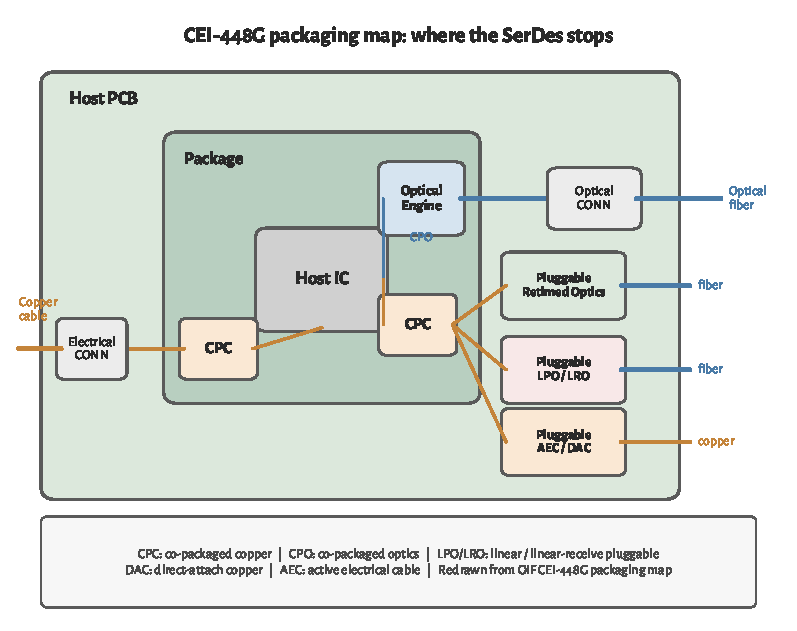
\includegraphics[width=\linewidth]{figures/fig_oif_448g_package.pdf}
\caption{CEI-448G packaging map (redrawn). CPC brings copper to the package edge;
CPO puts an optical engine in the package; faceplate cages take retimed optics,
LPO/LRO, or AEC/DAC. Same host IC, different SerDes reach and EQ burden.
\label{fig:oif-448g-package}}
\end{figure}

\paragraph{What ships today on that map (224G / 200G Ethernet).}
Before the 448G fork, every branch of \Cref{fig:oif-448g-package} already has a
shipping answer at the CEI-224G / IEEE 802.3dj lane rate. Faceplate ports run eight
224~Gb/s PAM4 lanes into 1.6~Tb/s OSFP-class modules (retimed DSP modules still
dominant; LPO and LRO gaining share where host COM and TDECQ close,
\Cref{sec:224g-deploy}). Copper inside the rack uses DAC, ACC, and AEC at the
same SerDes generation. CPO engines shipping with Tomahawk~6 and Quantum-X class
switches are typically \emph{200~Gb/s per optical channel} on 100G/200G SerDes
into microring banks with external lasers (\Cref{sec:cpo-status}): same packaging
map, one generation behind the 448G electrical debate. KP4 FEC, CEI-224G-Linear
for LPO, and KP4 pre-FEC BER near $2.4\times10^{-4}$ are the settled
electrical/optical contract (\Cref{sec:224g,sec:eye-budget,sec:kp4}). The rest of
this section is about what breaks when you try to double that lane rate on the
same shoreline.

So the ``448G debate'' is really two linked questions: can the \emph{electrical}
shoreline run PAM4 at 224~GBd, and can the \emph{optical} \term{PMD} modulate and detect
at the same symbol rate? \Cref{fig:448g-paths} maps the three dominant
architectures and the baud rate at each hop.

\begin{figure}[ht]
\centering
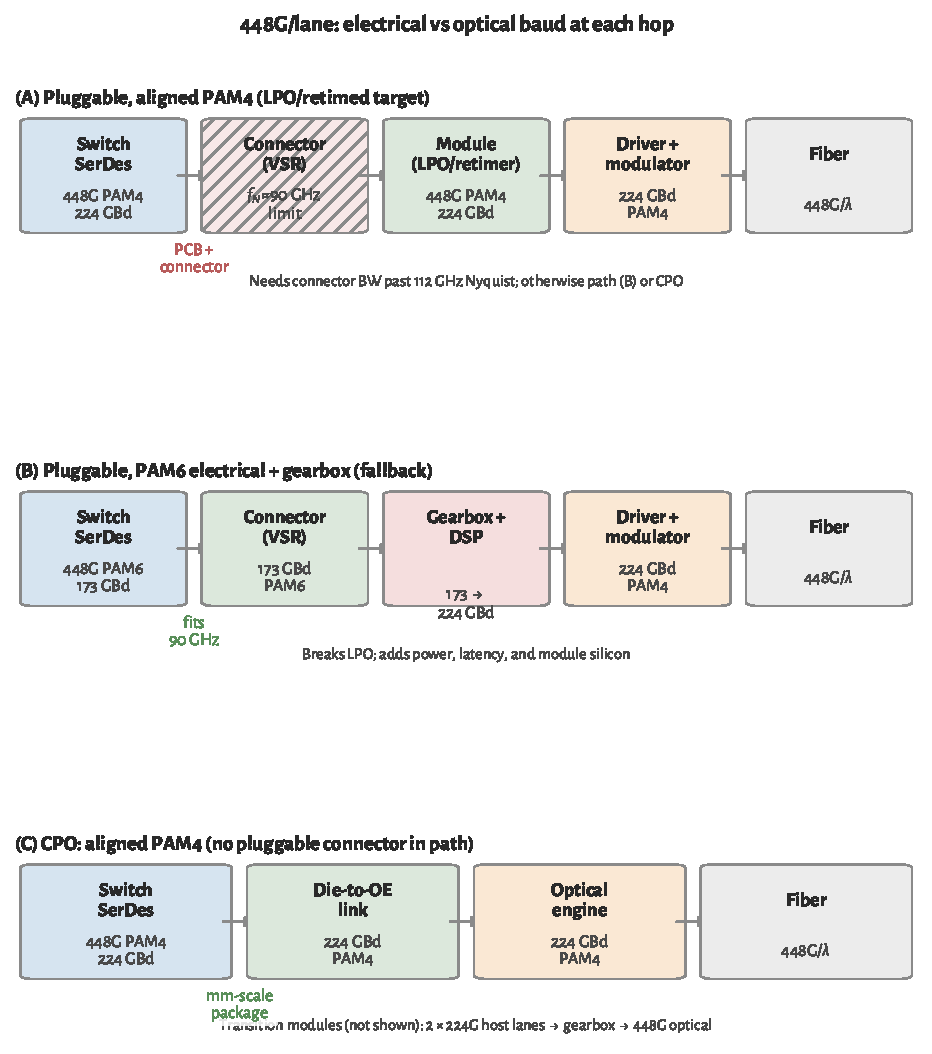
\includegraphics[width=\linewidth]{figures/fig_448g_paths.pdf}
\caption{448G/lane signal paths: aligned pluggable PAM4 (connector-limited),
         PAM6 electrical with module gearbox (LPO incompatible), and CPO or
         gearboxed 224G transition.\label{fig:448g-paths}}
\end{figure}

\begin{table}[ht]
\centering
\caption{PAM-$M$ options at 448~Gb/s/lane (OIF CEI-448G framework, pre-FEC
         line-rate target).\label{tab:448-mod}}
\begin{tabular}{@{}lrrrr@{}}
\toprule
Scheme & Symbol rate & $f_N$ & UI & SNR penalty vs.\ PAM4 \\
\midrule
PAM4 & 224~GBd   & 112~GHz & 4.5~ps & 0~dB \\
PAM6 & 173~GBd   & 87~GHz  & 5.8~ps & $\approx$2~dB \\
PAM8 & 149~GBd   & 75~GHz  & 6.7~ps & $\approx$4--5~dB \\
\bottomrule
\end{tabular}
\end{table}

\paragraph{FEC overhead and the SNR budget.}

At 224G, IEEE and CEI both lean on \term{KP4} FEC: Reed--Solomon RS(544,514) from
802.3 Clause~91, with coding overhead $30/544\approx5.5\%$ and a pre-FEC BER
target near $2.4\times10^{-4}$ for optical PHYs~\firstcite{ieee8023dj,cei448}. Post-FEC
the corrected BER target is $10^{-15}$ class. The line rate on the wire is higher
than the MAC/info rate: a 200~Gb/s Ethernet lane (802.3dj) runs PAM4 at 112~GBd
($224$~Gb/s raw) and delivers $\approx$211~Gb/s of payload after KP4, rounded to
200~Gb/s at the MAC.

448G pushes FEC harder. CEI-448G lists pre-FEC BER $10^{-4}$ as the working target
(same as prior CEI generations) but notes that $10^{-4}$ at $\ge$40~dB channel loss
may not close without a \emph{stronger} code than KP4~\firstcite{cei448}. PAM6 adds
$\sim$2~dB SNR penalty on top, so workshop assumptions often pair PAM6 with
\term{MLC}\firstterm{MLC} and higher-overhead FEC ($\sim$12\%) for a fair comparison to PAM4 with KP4~\firstcite{huawei448}.
\Cref{tab:448-fec} summarizes the landscape (OH\firstterm{OH} = coding overhead); 448G codes are not finalized
(see caption for sources).

\begin{table*}[ht]
\refstepcounter{table}\label{tab:448-fec}%
\centering
\setlength{\tabcolsep}{5pt}%
\begin{tabular}{@{}p{0.19\linewidth}p{0.15\linewidth}p{0.08\linewidth}p{0.49\linewidth}@{}}
\toprule
Context & FEC & OH & Role at 448G/lane \\
\midrule
802.3dj / 224G & KP4 RS(544,514) & 5.5\% &
  Baseline; pre-FEC BER near 2.4e-4. \\
CEI-448G, PAM4 elec. & KP4 or stronger & 5.5\%+ &
  Target pre-FEC 1e-4; KP4 may fail on 40~dB-class channels. \\
CEI-448G, PAM6 elec. & MLC + strong RS & 12\% &
  Offsets PAM6 SNR penalty; adds latency (workshop assumption). \\
448G optical demos & HD-FEC / product & 10--15\% &
  3.2T TFLN demo threshold; not necessarily host FEC. \\
FEC architecture & end-to-end vs.\ terminated & n/a &
  448G may need dedicated electrical inner code. \\
\bottomrule
\end{tabular}
\par\medskip
{\raggedright\footnotesize\textbf{Table~\thetable.} FEC at 448G/lane (448G codes provisional).\par}
\end{table*}
Sources: 802.3dj/KP4 baseline~\firstcite{ieee8023dj}; CEI-448G electrical
targets ~\firstcite{cei448}; PAM6 FEC assumption~\firstcite{huawei448}; optical
\firstterm{HDFEC} demo~\firstcite{tfmln32t}.

Higher FEC overhead feeds back into the modulation debate: every extra parity bit
raises the line rate and Nyquist frequency, which hurts a bandwidth-limited copper
channel. That is one reason PAM6 (lower baud) and stronger FEC get paired, and why
CPO (shorter electrical path) keeps PAM4 attractive.

\paragraph{Electrical SerDes: feasible, but the channel is the gate.}

448G SerDes themselves are widely treated as feasible on advanced CMOS
($\le$N3/N2): ADC/DAC DSP transmitters and receivers demonstrated at 224~Gb/s are
the template, and coherent-optics SerDes with $\sim$100~GHz class AFE at 200~GBd
is cited as encouraging precedent for doubling to 448G-PAM4~\firstcite{cei448}. Synopsys
and others have published channel simulations showing margin for both PAM4 and PAM6
on 224G-class channels when equalization and FEC scale with the modulation
order~\firstcite{synopsys448}. Power targets cluster around 0.5--2.5~pJ/bit at 448G,
similar in spirit to 224G scaling.

The blocker is not the PLL or the DAC; it is the \emph{passive channel}. Connector
bandwidth near 90~GHz forces a fork:

\begin{enumerate}
  \item \textbf{Fix the channel for PAM4:} new high-density connectors, shorter
        reach, skip-layer PCBs, cabled-host internal twinax. Simulations show
        passive CPC reach up to $\sim$1.2~m at 448G-PAM4 under optimistic
        connector assumptions~\firstcite{cei448}. This path preserves electrical/optical
        format alignment and keeps LPO/LRO architectures viable (\Cref{ch:networking}).
  \item \textbf{Keep the channel, change modulation:} PAM6 at 173~GBd fits a
        90~GHz channel but adds $\sim$2~dB SNR penalty and pushes the host toward
        stronger FEC than KP4. PAM8 relaxes bandwidth further at $\sim$4--5~dB
        penalty~\firstcite{cei448}.
  \item \textbf{Bypass the bad channel:} co-packaged optics with millimeter-scale
        die-to-OE links. Host 448G-PAM4 SerDes drives the optical engine directly;
        the pluggable connector never sees 224~GBd~\firstcite{cei448}.
\end{enumerate}

If electrical PAM6 wins on the PCB but optics stay at PAM4, the module needs a
\term{gearbox} (rate/format conversion) in the retimed path. That adds power,
latency, and silicon area, and it breaks linear pluggable optics: LPO requires the
host electrical waveform to match what the optical modulator expects~\firstcite{cei448,lpo}.
First 448G optical modules may therefore ship with gearboxed 224G SerDes (two 224G
lanes per 448G optical lane) before native 448G electrical I/O is
ready~\firstcite{huawei448}.

\paragraph{Optical modulation at 224~GBd: hard, but no longer hypothetical.}

On the optics side, the industry assumption is still IM/DD PAM4 at $\approx$224~GBd
for 448~Gb/s per $\lambda$~\firstcite{cei448,tfmln32t}. That requires roughly 112~GHz
class electro-optic bandwidth in the modulator (and comparable photodiode/TIA
bandwidth in the receiver), plus a driver with enough linear swing and RF BW.
By 2025--26 that stack exists in demos and, increasingly, in announced commercial
parts: silicon rings and MZMs with peaking, TFLN MZMs past 100~GHz EO bandwidth,
EMLs still owning volume at 200G/lane, and SiGe drivers / Ge receivers catching up.
The snapshot below is the state of play; device sections later unpack each family.

\begin{itemize}
  \item \textbf{Silicon microring modulators:} resonant, compact modulators for
        dense WDM and CPO (\Cref{sec:siring}). OFC 2026 demos reach 224--416~Gb/s
        PAM4 with inductive peaking~\firstcite{ring224,ring400}.
  \item \textbf{Silicon Mach--Zehnder modulators:} the broadband, non-resonant
        counterpart to microrings (\Cref{sec:simzm}). OFC 2026 demos reach
        400G/lane PAM4 with SiGe drivers~\firstcite{simzm400}.
  \item \textbf{EML:} integrated DFB + EAM remains the default through 200G/lane
        for DR/FR pluggables: one chip, low chirp, mature supply chain.
  \item \textbf{TFLN MZM:} thin-film lithium niobate Mach--Zehnder modulators with
        CW lasers exceed 100~GHz EO bandwidth and are the leading path to native
        224~GBd IM/DD (\Cref{sec:tfln-mzm}). A 3.2~Tb/s system (eight
        $\times$225~GBd PAM4 lanes) with 3~nm CMOS SerDes and TFLN modulators over
        2~km \term{FR8}/\term{DR8}\firstterm{FR8DR8} was reported in 2025~\firstcite{tfmln32t}.
  \item \textbf{Drivers:} commercial modulator drivers with $>$120~GHz RF BW for
        400G PAM4 EML/MZM/TFLN platforms appeared in 2026~\firstcite{macom448}.
  \item \textbf{Receivers:} Ge/Si PIN and APD photodiodes above 100~GHz and 224G
        TIAs exist (\Cref{sec:pd-tia,sec:rxtech}); the receive side is not the long pole relative
        to modulator/driver bandwidth at 448G.
\end{itemize}

\paragraph{Silicon microring and microdisk modulators.}
\label{sec:siring}

A microring modulator (MRM)\firstterm{MRM} wraps a phase-shifter waveguide into a closed loop
coupled to a straight \emph{bus} waveguide. A \emph{microdisk} is the same idea in
disk form: a pillar cavity evanescently coupled to the bus, often with a wider free
spectral range (FSR)\firstterm{FSR} in a smaller footprint. Both are resonant filters as well as
modulators: when the input wavelength sits on resonance, drop-port power is high;
off resonance it is rejected. Data modulation shifts the resonance (carrier
depletion or injection in an embedded pn junction) or detunes the laser relative
to a fixed ring, mapping voltage to intensity at the through or drop port.

The central design trade is \emph{photon lifetime versus bandwidth}. A high-$Q$
ring stores photons longer, which improves modulator efficiency ($V_\pi$) but narrows
the optical passband and creates an electrical bandwidth ceiling through the
RC-limited junction. Coupling strength, ring radius, and whether the device
operates in under-coupled or over-coupled regime set $Q$, extinction, and the
electro-optic (EO) roll-off. That trade does not appear in broadband Mach--Zehnder
modulators (\Cref{sec:simzm}).

Three constraints dominate ring modulator design at 100--400G per $\lambda$.
First, EO bandwidth: the junction RC roll-off is often below the target Nyquist
frequency, so inductive peaking (T-coils on the drive path), optimized detuning
from resonance, and compact RLC co-design extend EO BW without widening the ring
so much that $Q$ collapses~\firstcite{ring224,ring400}. Production CPO rings
target 50--90~GHz; conference demos report 90--110+~GHz with aggressive
peaking~\firstcite{ring224,ring400,ring256}. Second, wavelength alignment: ring
resonance drifts roughly 10~GHz/\textdegree C in silicon, so each $\lambda$ in a
WDM bank needs the laser or the ring tuned onto the modulator resonance
(\Cref{ch:wdm,sec:locking-techniques}). Thermal crosstalk from neighbors shifts
resonances in dense arrays, which is why fleet validation must include corner
temperature and adjacent-channel heating
(\Cref{sec:thermal-xtalk,ch:validation}). Third, optical loss and FSR: ring radius
sets FSR ($\Delta\lambda$ between adjacent resonances). Microdisk and
\emph{Euler} ring layouts widen FSR so more channels fit under one free spectral
range without collisions~\firstcite{ring256}, while residual coupling loss and
on-resonance insertion loss (often 1--3~dB class per modulator) eat link budget.

Integration is where rings win. A single SOI die can pack dozens of ring
modulators and filters for CW-WDM (\Cref{ch:wdm,sec:cwwdm}), each fed by one
wavelength from an external comb or multi-wavelength ELS (\Cref{ch:lasers}). The
photonic engine co-packaged with a switch ASIC (Broadcom Bailly/Davisson, NVIDIA
Quantum-X/Spectrum-X, \Cref{sec:cpo-status}) uses microring modulators at
200~Gb/s per channel today. Fiber count stays low because many $\lambda$ share one
waveguide; area and modulator count scale with WDM order rather than with
faceplate port count.

State of the art in 2025--26 shows how far that peaking path has been pushed.
Inductive and wavelength tuning carried silicon MRMs to 224~Gb/s PAM4 at 90~GHz
EO BW~\firstcite{ring224}. T-coil-peaked designs report 416~Gb/s PAM4
($\approx$208~GBd) with $>$110~GHz 1-dB EO BW and TDECQ 2.88~dB at
1~Vpp~\firstcite{ring400}. Euler microdisk rings show 256~Gb/s PAM4 with
$>$67~GHz EO BW and 3~THz FSR in O-band~\firstcite{ring256}. These are lab and
conference results, but they match the 200G/lane CPO shipping point and probe
448G-class lane rates when paired with sufficient electrical drive.

The platform choice is a packaging and control decision as much as a bandwidth
one. Prefer rings when many $\lambda$ must fit on one PIC and modulator area
dominates: CPO WDM engines, scale-up optical I/O, and any architecture that already
budgets for wavelength locking (\Cref{ch:wdm,ch:networking}). Prefer a silicon MZM
for single-$\lambda$ DR/FR where a flat passband avoids lock loops
(\Cref{sec:simzm}). Prefer TFLN when you need native 224~GBd in a pluggable and
ring thermal control at fleet scale looks harder than hybrid assembly
(\Cref{sec:tfln-mzm}).

\paragraph{Silicon Mach--Zehnder modulators.}
\label{sec:simzm}

Silicon photonics builds the Mach--Zehnder modulator (MZM)\firstterm{MZM} as a push-pull
interferometer on a silicon-on-insulator (SOI)\firstterm{SOI} rib or strip waveguide. Phase
shifters in each arm use \emph{carrier depletion} in an embedded pn junction:
reverse bias pulls carriers out of the waveguide core, lowering refractive index
and shifting optical phase. Intensity modulation comes from recombining the arms
at a 3-dB coupler, so chirp stays low compared with directly modulated lasers
(\Cref{ch:lasers}).

Three constraints mirror every high-speed MZM, but silicon's weak electro-optic
coefficient ($\Delta n$ per volt is far smaller than lithium niobate) sets the
numbers. The optical $S_{21}$ response must span the Nyquist frequency
($\approx$56~GHz at 112~GBd, 112~GHz at 224~GBd); junction capacitance, series
resistance, and traveling-wave electrode (TWE) microwave loss set the roll-off.
Production Si MZMs for 100--200G/lane modules typically quote 70--100+~GHz 3-dB
BW; differential-drive layouts and compact 300-mm platforms report 80--95~GHz
class results~\firstcite{simzmdiff,simzmcompact}. $V_\pi L$ for carrier-depletion
Si is often $\approx$1.5--2.5~V$\cdot$cm, so millimeter-scale devices need
2--4~V peak-to-peak drive at the target baud inside the linear range of a SiGe
or BiCMOS modulator driver (448G-class drivers exceed 120~GHz RF
BW)~\firstcite{macom448}. Unlike resonant rings, an MZM is broadband, so WDM
channels do not fight thermal lock (\Cref{ch:wdm}); the cost is length:
mm-scale shifters and splitters add 2--4~dB on chip, and the device is far larger
than a ring, which matters in dense CPO tiles.

Integration is the main reason Si MZM survives competition from EML and TFLN.
The modulator shares a die with Ge photodiodes, fiber grating couplers or edge
couplers, monitors, and (in WDM products) MUX/de-MUX filters, all in a CMOS
foundry-compatible flow. An external CW DFB or ELS (\Cref{ch:lasers}) couples in
through a spot-size converter; the RF driver is usually a separate die wire-bonded
or 2.5D packaged next to the PIC, the same assembly style as TFLN modules but
without bonding a second optical material stack.

State of the art in 2025--26: Si MZMs are the default modulator in 100G/lane and
200G/lane DR/FR silicon-photonics\firstterm{SiPh} transceivers. Pushing to 400G/lane IM/DD was open
until OFC 2026, when Coherent reported 400~Gb/s PAM4 per lane with a Si MZM and
commercial SiGe driver (2.5~V swing)~\firstcite{simzm400}. The same conference
cycle showed a 500~$\mu$m compact MZM on a 300-mm platform with 94.7~GHz median EO
BW and 2.4~dB on-chip insertion loss~\firstcite{simzmcompact}, and a
differential-drive MZM with 81.8~GHz 3-dB BW with eyes to 100~GBd
PAM8~\firstcite{simzmdiff}. These are lab and conference demos, not shipping
modules, but they close the headline lane-rate gap with ring modulators while
keeping a flat passband that rings only match with tight wavelength control
(\Cref{sec:siring}).

\paragraph{Thin-film lithium niobate Mach--Zehnder modulators.}
\label{sec:tfln-mzm}

\term{TFLN}\firstterm{TFLN} refers to a sub-micrometer slice of lithium niobate bonded to a
silicon or silica handle wafer. Compared with bulk LN, the tight optical mode
confinement shrinks electrode gap and interaction length, which cuts the
half-wave voltage--length product $V_\pi L$ while keeping a wide
\term{electro-optic}\firstterm{EO} (EO) bandwidth. The modulator is a Mach--Zehnder
interferometer (MZM): a \term{Pockels} phase shifter in each arm, driven in
push-pull, converts RF voltage on a \term{traveling-wave electrode}\firstterm{TWE} (TWE) into
intensity at the output coupler.

Three design constraints set whether a TFLN MZM can run at 224~GBd PAM4
($f_N\approx112$~GHz). EO bandwidth, measured as the $S_{21}$ roll-off of optical
response versus RF drive, must clear that Nyquist: production-class devices quote
$\gtrsim$110~GHz 3-dB BW, and research devices with low-$k$ underfill or advanced
TWE layouts extrapolate toward 200+~GHz~\firstcite{tfln390,tfln200mm}.
$V_\pi L\approx1$--2~V$\cdot$cm is typical, so a 5--7~mm device gives
$V_\pi\approx1.5$--2~V that must fit inside the linear swing of a SiGe or InP
driver at 112~GHz class~\firstcite{macom448,tfln224}. Along the TWE, microwave and
optical group indices must match or bandwidth collapses; low-loss underfill,
narrow-gap CPW or co-planar layouts, and transparent conductive oxide (TCO)
electrodes trade insertion loss against efficiency~\firstcite{tfln224,tfln390}.

Demonstrated IM/DD results on TFLN MZMs include 224~Gb/s PAM4 at 108~GHz EO BW
(O-band, $V_\pi L=1.02$~V$\cdot$cm)~\firstcite{tfln224} and 390~Gb/s PAM8 on the
same dual-band chip (extrapolated 220~GHz BW, sub-fJ/bit in lab)~\firstcite{tfln390}.
System-level proof came with eight $\times$225~GBd PAM4 lanes over 2~km using
3~nm SerDes and packaged TFLN modulators~\firstcite{tfmln32t}. Commercial
suppliers (HyperLight, Lumiphase, and foundry lines on 200-mm silicon) now ship
110~GHz-class packaged MZMs aimed at 200--240~GBd signaling~\firstcite{hyperlight110,tfln200mm}.

Integration looks unlike monolithic silicon photonics. A CW DFB or ELS feeds the
TFLN chip through a Si/SiN coupler; the RF driver sits on a separate die,
wire-bonded or flip-chip mounted with matched 50~$\Omega$ lines. Hybrid Si--LN
platforms (silicon waveguides, LN overlay) were demonstrated early for 100G/lane
and remain a template for co-packaged assemblies~\firstcite{he2019}. The laser
is not on the TFLN chip, so alignment, fiber attach, and thermal bias of the MZM
quadrature point become validation items (\Cref{ch:validation}).

\paragraph{EML and the electro-absorption modulator.}
\label{sec:eml-eam}

An \term{EML} integrates a DFB laser with an \term{EAM}\firstterm{EAM}
(electro-absorption modulator) on one InP chip. The EAM is a reverse-biased
absorption region: voltage shifts the band edge (Franz-Keldysh or quantum-confined
Stark effect), attenuating light with far less chirp than direct current modulation
(\Cref{sec:chirp-dispersion}).

EMLs dominate 100G/lane and 200G/lane DR/FR pluggables because they are single-chip,
mature in supply chain, and match $\sim$70--100~GHz class EO bandwidth
(\Cref{tab:tx-modulator}). The design limits that show up in validation are EAM
bias and aging (bias sets extinction and chirp; aging drifts the curve and shows
up as TDECQ/RLM creep, \Cref{ch:validation,ch:reliability}), driver swing (a few
volts inside the linear absorption region; 448G-class EML drivers appeared
alongside MZM drivers in 2026~\firstcite{macom448}), and thermal headroom
(uncooled datacom is standard; slope efficiency and bias must stay in range
across case temperature).

EML wins on cost and integration through 200G/lane. Above that, external modulators
(Si MZM, TFLN, rings with CW laser) chase bandwidth and chirp headroom
(\Cref{sec:simzm,sec:tfln-mzm,sec:siring}).

\paragraph{Modulator drivers: requirements, records, outlook.}
\label{sec:drivers}

Every external modulator (Si MZM, TFLN, ring, EAM) needs an RF path that delivers
enough \emph{linear} swing at the target baud. That path is either a dedicated
SiGe\firstterm{SiGe}/BiCMOS\firstterm{BiCMOS} \emph{modulator driver} die, or (for LPO) the host SerDes itself.
Laser \emph{bias} drivers are a different circuit and a different noise budget
(\Cref{sec:laser-drivers}). Do not share the modulator driver's switching returns
with the CW bias rail.

\paragraph{What the driver must deliver.}
At 224~GBd PAM4 the symbol Nyquist frequency is 112~GHz, so a usable driver is
not just ``fast enough on paper.'' It needs RF bandwidth roughly
$\gtrsim$100--120~GHz (3~dB) with flat gain and low group-delay ripple, output
swing matched to $V_\pi$ or EAM drive (often $\sim$1.5--3~V peak-to-peak,
differential or single-ended, part- and modulator-dependent), linearity good
enough that RLM and TDECQ stay inside the PMD budget when the optical path adds
its own compression (\Cref{sec:tdecq}), and return loss / matching into
50~$\Omega$ (or the designed modulator impedance) so bondwire and package
reflections do not eat the bandwidth you paid for on the die.
Distributed (traveling-wave) SiGe drivers dominate the high-BW niche: many
cascoded gain cells along an artificial transmission line. Lumped drivers win on
area and power at lower baud. Flip-chip bumped die and short wirebonds matter as
much as $f_T$: a 120~GHz die behind a long bond loop is a 70~GHz module.

\paragraph{Record and commercial snapshot (2025--26).}
\Cref{tab:driver-records} separates research demos (often with offline DSP) from
shipping or announced commercial parts aimed at 1.6T/3.2T modules. Commercial
anchors: MACOM's MAOM-025408 MZM and MAOM-022404 EML drivers ($>$120~GHz RF BW,
OFC~2026)~\firstcite{macom448}; Semtech's GN1877/GN1887 224G quad/octal family for
LPO/LRO/CPO across SiPh, InP, and TFLN~\firstcite{semtech224}. Research anchors:
a 130~nm SiGe distributed driver at 105.7~GHz BW and 2.25~V swing running
232~GBd PAM4 into TFLN (offline DSP)~\firstcite{rfic460drv}; OFC~2026 co-designed
engines at 210~GBd / 420~Gb/s PAM4 (TFLN TOSA)~\firstcite{ofc420tosa}, 180~GBd
PAM4 (InP MZM + EML-class driver)~\firstcite{ofc180drv}, and differential
SiGe+TFLN at 140~GBd PAM8 / 1.4~pJ/bit~\firstcite{tflndiffdrv}; plus the Si MZM
postdeadline with a commercial SiGe driver at 400~Gb/s/lane and 2.5~V
swing~\firstcite{simzm400}.

\begin{table*}[ht]
\refstepcounter{table}\label{tab:driver-records}%
\centering
\setlength{\tabcolsep}{3pt}%
\footnotesize
\begin{tabular}{@{}p{0.24\linewidth}p{0.12\linewidth}p{0.14\linewidth}p{0.16\linewidth}p{0.26\linewidth}@{}}
\toprule
Part / paper & Process & RF BW & Rate / swing & Note \\
\midrule
MACOM MAOM-025408 (MZM) & SiGe & $>$120~GHz & 448G-class PAM4 & Commercial; SiPh MZM \\
MACOM MAOM-022404 (EML) & SiGe & $>$120~GHz & 448G-class PAM4 & Commercial; EML / TFLN \\
Semtech GN1877 / GN1887 & --- & 224G-class & 224~Gb/s/lane & Quad/octal; LPO path \\
RFIC 2026 distributed drv & 130~nm SiGe & 105.7~GHz & 232~GBd; 2.25~V & Research; TFLN; offline DSP \\
OFC 2026 Si MZM + SiGe & commercial SiGe & (drv-limited) & 400~Gb/s/lane; 2.5~V & Postdeadline Th4A.4 \\
OFC 2026 TFLN TOSA & co-designed & --- & 210~GBd / 420~Gb/s & Driver+TFLN engine \\
OFC 2026 InP MZM + EML drv & InP + SiGe-class & 76~GHz MZM & 180~GBd PAM4 & Co-packaged engine \\
Nokia/Bell Labs hybrid & SiGe + TFLN & --- & 140~GBd PAM8; 1.4~pJ/bit & Diff.\ drive; low $V_\pi L$ \\
\bottomrule
\end{tabular}
\par\medskip
{\raggedright\footnotesize\textbf{Table~\thetable.} Modulator-driver snapshot (c.~2026).
Commercial rows are vendor announcements (bandwidth/swing as published); research
rows often use offline DSP and short RF interconnects. ``448G-class'' means aimed at
$\sim$400--448~Gb/s/lane PAM4 modules, not a CEI compliance claim. Sources cited in
the paragraph above.\par}
\end{table*}

\paragraph{LPO and the host-as-driver path.}
For \term{LPO}, the host SerDes (or a linear driver in the module with no retimer)
is the modulator driver. Waveform fidelity is end to end: host FFE, connector ISI,
driver/modulator nonlinearity, and TIA all land in TDECQ and pre-FEC BER
(\Cref{sec:equalization,sec:tdecq,sec:conditioning}). That is why linear-optics
driver families (e.g.\ Semtech's 224G set) advertise CEI-224G-Linear host EQ and
tunable swing: the module cannot clean up what the host launches~\citehref{semtech224}{Semtech 224G}.
Retimed modules hide some of this behind DSP; they also burn the watts LPO was
meant to save.

\paragraph{Outlook.}
Driver roadmaps are no longer waiting on papers alone. Commercial 448G-class
parts are shipping as dies: MACOM's $>$120~GHz MZM and EML drivers (OFC 2026) are
the clearest public 400G/lane announcement~\citehref{macom448}{MACOM}, while
research benches already run past 200~GBd on short RF paths. Expect a short
period where optics and drivers lead host SerDes, so gearboxed 224G electrical
into 448G optical remains common (\Cref{sec:gearbox,sec:448g}). The hard problems
are packaging (bondwire, FAU, faceplate connectors), co-design of peaking with
modulator $S_{21}$, and LPO cases where driver linearity and host COM sit beside
TDECQ as first-order validation items (\Cref{sec:com,sec:prod-corners}). After
the driver, the next ceilings are modulator EO bandwidth and the PD/TIA noise
stack (\Cref{sec:simzm,sec:tfln-mzm,sec:siring,sec:pd-tia,sec:rxtech}).

\keyidea{A 448G-class modulator driver is a $>$100~GHz linear SiGe amp with swing
matched to $V_\pi$, not a SerDes pin. Commercial dies now claim $>$120~GHz for
MZM/EML/TFLN; research shows $\sim$230~GBd on co-designed benches. Package and
modulator match set the real ceiling; LPO makes the host the driver.}

\paragraph{Gearboxes: when electrical and optical rates diverge.}
\label{sec:gearbox}

A \term{gearbox}\firstterm{gearbox} converts lane rate or modulation format between
electrical and optical domains. The 448G transition often uses \emph{two} 224G
electrical lanes into one 448G optical lane (\Cref{fig:448g-paths,sec:448g}) when
host SerDes or connectors lag optics.

Gearboxes add power, latency, and silicon area. They also break strict LPO: the host
waveform no longer matches what the optical lane carries, so a retimed or
half-retimed module is required~\firstcite{cei448,lpo}. Expect gearboxed 3.2T modules
before native 448G electrical I/O and matched VSR connectors land in volume.

Putting the platforms side by side, \Cref{tab:tx-modulator} summarizes the trade
space at 100--400G per $\lambda$; \Cref{sec:siring,sec:simzm,sec:tfln-mzm,sec:eml-eam}
expand each path. Through 200G/lane DR, EML still leads on cost and single-chip
integration. Silicon rings and MZMs lead in CPO where area and CMOS fab matter,
with Si MZM preferred for flat single-$\lambda$ DR/FR and rings preferred for dense
WDM. TFLN leads when you need $\gtrsim$100~GHz EO BW with low chirp for native
224~GBd PAM4 in a pluggable or NPO module and silicon cannot close the 112~GHz
Nyquist without heavy peaking.

\begin{table*}[ht]
\refstepcounter{table}\label{tab:tx-modulator}%
\centering
\setlength{\tabcolsep}{4pt}%
\footnotesize
\begin{tabular}{@{}p{0.11\linewidth}p{0.10\linewidth}p{0.14\linewidth}p{0.08\linewidth}p{0.18\linewidth}p{0.33\linewidth}@{}}
\toprule
Platform & EO BW & Per-$\lambda$ demo & Chirp & Integration & Typical use \\
\midrule
Si microring & 90--110~GHz & 224--416~Gb/s PAM4 & low & monolithic SiPh & CPO, WDM \\
Si MZM & 70--100+~GHz & 400~Gb/s PAM4 & low & monolithic SiPh & DR/FR, CPO \\
TFLN MZM & 108--110+~GHz & 224--390~Gb/s PAM4/8 & very low & hybrid + driver die & 400G/lane pluggable, FR \\
EML & 70--100~GHz & 200~Gb/s PAM4 & low & single InP chip & DR/FR to 200G/lane \\
\bottomrule
\end{tabular}
\par\medskip
{\raggedright\footnotesize\textbf{Table~\thetable.} IM/DD transmitter platforms at 100--400G per $\lambda$ (2026 snapshot).\par}
\end{table*}

The honest summary: \emph{modulating} at 224~GBd PAM4 is demonstrated in multiple
material systems when the electrical drive path is short and the driver is
dedicated (not a lossy meter of PCB plus OSFP connector). \emph{Modulating} at that
rate from a switch ASIC through a pluggable module is the harder system problem.
Silicon photonics rings without peaking still sit below the 112~GHz Nyquist needed
for 448G-PAM4; TFLN, EML, and peaked Si rings are the near-term paths. WDM
(\Cref{ch:wdm}) and CPO remain the architectural escape hatches: more
aggregate bits without forcing every electrical lane to 224~GBd on a lossy
shoreline.

\paragraph{Where the standards conversation stands.}
Electrical and Ethernet standards are climbing the same ladder on slightly
different clocks. OIF CEI owns the electrical I/O recipe; IEEE 802.3 owns how
Ethernet names the lane and the optical PMD. Neither has locked 448G modulation
yet.

\paragraph{OIF CEI (electrical I/O).}
No modulation order is locked yet in CEI-448G. PAM4 remains attractive if
connectors reach $\gtrsim$112~GHz and if optics stay on PAM4 (alignment for LPO,
lower FEC overhead, backward compatibility with 224G gear). PAM6 is the leading
compromise for bandwidth-starved host channels if connector progress
stalls~\firstcite{cei448,cignal448}. Electrical IAs target a 2026--28
window~\firstcite{cei448}.

\paragraph{IEEE 802.3 (Ethernet PHY/MAC).}
Ethernet standards trail CEI slightly but follow the same lane-doubling cadence.
\Cref{tab:ieee-lane} is the map as of mid-2026.

\begin{table}[ht]
\centering
\caption{IEEE 802.3 lane-rate generations.\label{tab:ieee-lane}}
\begin{tabular}{@{}llll@{}}
\toprule
Project & Status & Eth.\ lane & PHY line \\
\midrule
802.3df & Feb 2024 & 100~Gb/s & $\approx$112G PAM4 \\
802.3dj & SA ballot 2026 & 200~Gb/s & $\approx$224G PAM4 \\
802.3 400G/lane SG & Mar 2026 & 400~Gb/s & $\approx$448G \\
\bottomrule
\end{tabular}
\end{table}

\textbf{802.3df} (approved February 2024) defined 200/400/800~Gb/s Ethernet using
\textbf{100~Gb/s lanes} (112~GBd PAM4 class). \textbf{802.3dj} is the active
200~Gb/s-lane amendment: 200/400/800/1600~Gb/s Ethernet with PAM4 at 112~GBd,
KP4 FEC, and a large PHY portfolio (copper and IM/DD optics). The draft cleared
802.3 working-group recirculation ballot in February 2026 and entered IEEE
Standards Association ballot; approval is expected around late
2026~\firstcite{ieee8023dj,e4ai448}.

\textbf{400~Gb/s per lane} is the next Ethernet milestone. The \term{Ethernet for
AI} (E4AI) ad hoc incubated demand for 3.2~Tb/s ports and 400G/lane
signaling~\firstcite{e4ai448}. A call for interest in March 2026 led to an IEEE 802.3
\textbf{400~Gb/s/lane Signaling Study Group} (chartered 13 March 2026) to draft a
PAR for electrical interconnects and single-mode fiber reaches up to
500~m~\firstcite{ieee400gpl}. The proposed scope has two tracks: a fast track for
400/800/1600~Gb/s on 400G/lane copper and IM/DD optics (scale-up, intra/inter-rack),
and a follow-on phase for \textbf{3.2~Tb/s} and additional PHYs~\firstcite{e4ai448,ieee400gpl}.
That aligns with OIF CEI-448G and industry 3.2T module work, with one naming
difference: IEEE quotes \textbf{400~Gb/s per lane} (MAC/info rate); CEI quotes
\textbf{448~Gb/s} (line rate including FEC overhead). They refer to the same
generation.

Until native 448G host SerDes and matched connectors land, expect a transition
generation that gearboxes 224G electrical lanes into 448G optical lanes
(\Cref{fig:448g-paths}), then a consolidation generation with 400G/lane Ethernet
PHYs where electrical and optical both run PAM4 at 224~GBd end to end.

\keyidea{IM/DD is intensity in, power out, with FEC and DSP closing the gap that
PAM4's SNR penalty opens. Master OMA, ER, chirp/dispersion, and pre-FEC BER and
you can reason about any short-reach link.}
